


\section{Descripción General del Desarrollo del Protocolo}
El protocolo criptográfico para evitar duplicados almacenados en la nube, es un proyecto que involucra la tecnología de software para ofrecer un funcionamiento eficiente y útil para las necesidades de los usuarios que se encuentran inmersos en el cómputo nube. 
Nuestro protocolo, se compone a su vez de diferentes módulos. Cada uno de ellos busca satisfacer: \\ 

\begin{itemize}

\item La seguridad de los archivos de los usuarios en la nube
\item Almacenamiento seguro en la sube
\item Conexión de diversos usuarios 
\item Ahorro en el consumo de espacio ofrecido en la nube 
\item Fácil acceso al almacenamiento de los archivos de los usuarios 

\end{itemize} 

Para lograrlo, el protocolo criptográfico se compone de diversos módulos que a su vez integran diferentes aplicaciones criptográficas. Dichos módulos serán detallados en las próximas secciones. 

\section{Servidor de Llaves}
El módulo Servidor de llaves tiene una función muy importante dentro del funcionamiento del protocolo criptográfico, ya que sin dicho servidor los usuarios no podrían conectarse para poder utilizar el servicio de almacenamiento seguro. 

\subsubsection{Objetivo}
\begin{itemize}
	\item Generar llaves certificadas para cifrar los archivos.
	\item Brindar seguridad ante ataques por fuerza bruta.
\end{itemize}

\subsubsection{Entradas}
\begin{itemize}
	\item El factor de ocultamiento (Proporcionado por el cliente)
	\item La clave privada del servidor \textit{d} , generada mediante el algoritmo RSA. 
\end{itemize}

El desarrollo de éste módulo, fué realizado mediante el lenguaje de programación Python en su versión 2.7. \\
Las librerías utilizadas para llevar acabo la implementación de éste módulo son: 

\begin{lstlisting}[language=Python,frame=single, keywordstyle=\color{blue},showstringspaces=false]
			import SocketServer
			import threading
			import time
			from rsagen import *
\end{lstlisting}

Para crear el socket utilizado en el servidor, ocupamos el modulo \textbf{socket} de Python, el cuál importamos desdse la librería \textbf{SocketServer}, dicho módulo simplifica la tarea de escribir servidores de red montados en el lenguaje de programación python. \\ La librería \textbf{threading} construye interfaces de subprocesamiento de nivel superior en la parte superior del thread.\\
La librería \textbf{time} disponible en Python proporciona funciones para trabajar con los tiempos y para convertir representaciones. \\
Finalmente,\textbf{ rsagen} es una implementación de Python RSA pura. Es compatible con el cifrado,  el descifrado, la firma, verificación de firmas y la generación de claves de acuerdo con PKCS \# 1 versión 1.5. Se puede utilizar como una biblioteca de Python, así como en la línea de comandos.
\\ \\ 

Una vez que importamos las bibliotecas pertinentes, se generan las llaves del servidor, tanto la pública \textit{(e)}, como la privada \textit{(d)}, para esto usamos el método \textit{gen\_rsa(usuario)}, es decir utilizamos RSA para la generación de llaves y para ello hacemos uso de \textit{rsagen}, donde ya viene la implementación de dicho algoritmo. \\ 

Posteriormente leemos el archivo \textit{n} y la llave privada \textit{d} del servidor.

	\begin{lstlisting}[language=Python,frame=single, keywordstyle=\color{blue},showstringspaces=false]
	usuario = 'server'
	gen_rsa(usuario)
	n = int(open("key_n_server.PEM", "r").read())
	d = int((open("key_d_server.PEM", "r").read())
	\end{lstlisting}

Para continuar, creamos un TCP Handler el cual utiliza el protocolo TCP de Internet, que proporciona transmisiones continuas de datos entre el cliente y el servidor.

 
\begin{lstlisting}[language=Python,frame=single, keywordstyle=\color{blue},showstringspaces=false]
#creo mi TCP Handler
class MiTcpHandler(SocketServer.BaseRequestHandler):
\end{lstlisting}


Ya que tenemos la conexión entre las dos partes ahora estamos listos para recibir los datos enviados por el cliente, lo que vamos a recibir se le llama factor de ocultamiento  \textit{x} esto nos ayuda a que el servidor quien va a realizar una firma a ciegas no sepa que es lo que este firmando, y no se entere de la información manejada, ya que tenemos este factor ahora si, el servidor se dispone a realizar la firma a ciegas \textit{y} para que pueda continuar con la creación de la llave para poder cifrar los archivos

\begin{lstlisting}[language=Python,frame=single, keywordstyle=\color{blue},showstringspaces=false]
       def handle(self):
        data= ""
        while data != "salir":
            #intento recibir informacion
            try:
                data= self.request.recv(65536)
                print data
                x = int(data)
                print "x:", x
                y = pow(x,d,n)
				#Devolvemos el mensaje al cliente
                print "y:", y
                self.request.send(str(y))
                time.sleep(0.1)
			
            #si hubo un error lo digo y termino el handle
            except:
                print "El cliente D/C o hubo un error"
                data="salir"
\end{lstlisting}

Obteniendo la firma a ciegas \textit{y} se la enviamos a nuestro cliente para que pueda continuar en la creación de la llave \textit{z}, esto se ve explicado mas adelante cuando se explique la interfaz.



%En la función handle mientras \textit{data} sea distinto de \textit{“Salir”} intentará recibir la información, imprimirá en pantalla \textit{“Nuevo Cliente Conectado”} 

			%\begin{figure}[H]
			%\centering
			%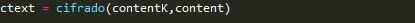
\includegraphics[width=14cm, height=10cm]{./images/servidor/04.jpg}
			%\caption{Conexión de Clientes}
			%\label{fig:6-1-4} 
			%\end{figure}



\section{Aplicación Criptográfica (Cifrado/Descifrado)}

%Éste módulo del protocolo es de suma importancia para ofrecer la seguridad de los archivos como se menciona anteriormente, ya que en éste módulo se lleva a cabo para blindar un archivo, es decir cifrarlo. 
%El desarrollo de éste módulo fue realizado en el lenguaje de programación Python versión 2.7.3. Además de que para la implementación del algoritmo de cifrado AES se utilizó principalmente la biblioteca criptográfica Pycripto 2.3. 

\subsection{Cifrado}
Éste algoritmo que forma parte de la aplicación criptográfica, se lleva a cabo del lado del cliente, dicho algoritmo de cifrado se encargará de brindar la seguridad a los archivos que los usuarios deseen almacenar en la nube. \\
El cifrado de archivos se lleva a cabo bajo la utilización del algoritmo de cifrado \textbf{AES} que proveé la librería criptográfica \textbf{PyCripto 2.3} propia del lenguaje \textbf{Python}. Ésta librería poseé la seguridad necesaria para satisfacer a los requerimientos del protocolo criptográfico.  \\ 

\subsubsection{Objetivo}
Proteger la información que se almacenará en la nube.

\subsubsection{Entradas}
	\begin{itemize}
		\item El archivo que se almacenará en la nube.
		\item La clave para poder cifrarlo, que en este caso es la llave \textit{(z)} generada por el cliente en el módulo anterior. 
	\end{itemize}

La implementación del algoritmo, se llevó a cabo de la siguiente manera: 

\begin{lstlisting}[language=Python,frame=single, keywordstyle=\color{blue},showstringspaces=false]
from random import randint
import socket
import hashlib
import hmac
import Crypto.Cipher.AES, Crypto.Util.Counter
import hmac
from rsagen import *
from Duplicidad import *
from django.core.files import File
from models import Hashes,Cipher
\end{lstlisting}

Siendo \textbf{haslib, Crypto.Cipher.AES, Crypto.Util.Counter, hmac} librerías criptográficas, es decir, utilizadas para llevar a cabo operaciones relacionadas con la implementación del algoritmo de cifrado \textit{AES} en sus 3 tipos de tamaños de claves \textit{(128, 192, 256 bits)}.\\ \\ 

\begin{itemize}

	\item Para poder comenzar el proceso de cifrado, es necesario obtener la clave que se utilizará para llevar a cabo el proceso. \\ Dicha clave se obtiene de la siguiente manera: 

	\begin{lstlisting}[language=Python,frame=single, keywordstyle=\color{blue},breaklines=true,showstringspaces=false]
 	contentK2 = open("llaves_clientes/key_z_"+filename+"_"+nom_user+".PEM", "rb").read()
	\end{lstlisting}

Abrimos el archivo \textbf{key\_z} y almacenamos su contenido en la variable \textbf{contentK}. Éste archivo contiene la clave que se necesita para poder cifrar el archivo que el usuario desea, dicha \textit{clave (z)} fue generada y escrita en este archivo en el módulo anterior. 

	\item Se crea un objeto de tipo \textit{AES} que almacenamos en la variable \textbf{cipher}, el cual contiene como parámetros la clave que obtuvo del archivo  \textbf{key\_z}, el modo de operación que se utilizará \textbf{(CTR)}, etc.
			
\begin{lstlisting}[language=Python,frame=single, keywordstyle=\color{blue},breaklines=true,showstringspaces=false]
cipher = Crypto.Cipher.AES.new(contentK2, Crypto.Cipher.AES.MODE_CTR, counter=ctr)
\end{lstlisting}

	\item Para cifrar el archivo, mandamos llamar al método \textbf{\textit{encrypt(m)}} \textit{(m almacena el contenido del archivo que se desea cifrar)} y almacenamos el resultado de dicho método en la variable \textbf{ctext.} y esta variable contiene el archivo cifrado por completo
			
	\begin{lstlisting}[language=Python,frame=single, keywordstyle=\color{blue},breaklines=true,showstringspaces=false]
		ctext = cipher.encrypt(m)
	\end{lstlisting}



\end{itemize}


\subsection{Descifrado}
Éste algoritmo que forma parte de la aplicación criptográfica, al igual que el cifrado, se lleva a cabo del lado del cliente, éste algoritmo será el encargado de que los usuarios puedan recuperar sus archivos originales, es decir, tomar de la nube aquel archivo que se encuentre cifrado y posteriormente descifrarlo para poder acceder a este archivo en su forma original. \\
El descifrado de archivos se lleva a cabo bajo la utilización del algoritmo de descifrado \textbf{AES} que, al igual que el cifrado lo proveé la librería criptográfica \textbf{PyCripto 2.3} propia del lenguaje \textbf{Python}.   \\ 

\subsubsection{Objetivo}
Descifrar los archivos almacenados de forma íntegra.

\subsubsection{Entradas}
	\begin{itemize}
		\item El archivo que se almacenó en la nube.
		\item La clave para poder descifrarlo, que en este caso es la llave \textit{(z)} generada por el cliente.
	\end{itemize}

La implementación del algoritmo, se llevó a cabo de la siguiente manera: 

\begin{itemize}
	\item Las librerías utilizadas para llevar a cabo el descifrado de archivos son las siguientes: 
			
\begin{lstlisting}[language=Python,frame=single, keywordstyle=\color{blue},breaklines=true,showstringspaces=false]
	from random import randint
	import socket
	import hashlib
	import hmac
	import Crypto.Cipher.AES, Crypto.Util.Counter
	from rsagen import *
	from Duplicidad import *
	from django.core.files import File
	from models import Hashes,Cipher
\end{lstlisting}

Siendo \textbf{Crypto.Cipher.AES, Crypto.Util.Counter}, librerías criptográficas, es decir, utilizadas para llevar a cabo operaciones relacionadas con la implementación del algoritmo de descifrado \textit{AES} en sus 3 tipos de tamaños de claves \textit{(128, 192, 256 bits)}. 

	\item Al igual que en el proceso de cifrado, para comenzar dicho proceso es necesario obtener la clave que se utilizará para el descifrado. Dicha clave se obtiene de la siguiente manera:  

\begin{lstlisting}[language=Python,frame=single, keywordstyle=\color{blue},breaklines=true,showstringspaces=false]
    contentK2 = open("llaves_clientes/key_z_"+filename+"_"+nom_user+".PEM", "rb").read()
\end{lstlisting}

Abrimos el archivo \textbf{key\_z} y almacenamos su contenido en la variable \textbf{contentK}. 

		\item El siguiente paso, es buscar en la base de datos el archivo que se va a descifrar y se guarda en una variable. 
			
\begin{lstlisting}[language=Python,frame=single, keywordstyle=\color{blue},breaklines=true,showstringspaces=false]
    buscar = Cipher.objects.filter(hash_c=doc).all()[0]
    file_c1 = File(buscar.docfile).read()
\end{lstlisting}

Una vez dentro del archivo, almacenamos el cifrado en la variable \textbf{textcifrado} para utilizarlo posteriormente. 

		\item Creamos un objeto \textit{AES} que almacenamos en la variable \textbf{ciphe}r, el cual contiene como parámetros la llave que obtuvo del archivo \textbf{key\_z }, el modo de operación que se utilizará para el descifrado\textbf{(CTR)}, etc.
			
\begin{lstlisting}[language=Python,frame=single, keywordstyle=\color{blue},breaklines=true,showstringspaces=false]
cipher = Crypto.Cipher.AES.new(contentK, Crypto.Cipher.AES.MODE_CTR, counter=ctr)
\end{lstlisting}


		\item Desciframos el archivo, mandamos llamar al método \textbf{\textit{decrypt(textcifrado)}}  y almacenamos el resultado de dicho método en la variable \textbf{plaintext}
		
\begin{lstlisting}[language=Python,frame=single, keywordstyle=\color{blue},breaklines=true,showstringspaces=false]
    	return cipher.decrypt(textcifrado)
\end{lstlisting}

		\item Para finalizar, mandamos escribir a un archivo \textbf{fname} \textit{(Es el nombre del archivo original del usuario)} el archivo tal y como estaba antes de cifrarlo. 
			
\begin{lstlisting}[language=Python,frame=single, keywordstyle=\color{blue},breaklines=true,showstringspaces=false]
	plaintext = descifrado(contentK2, textcifrado, iv)
    	outf = open("Descifrados/" + nom_user + "/" + filename, "wb")
   	outf.write(plaintext)
    	outf.close()
   	print "Mensaje Descifrado c1: "
\end{lstlisting}

\end{itemize}

\section{Interfaz Web}

En ésta sección, se encuentra el detalle de la implementación de los módulos anteriores dentro de una interfaz web.\\
Dicha interfaz se desarrolló bajo el sistema operativo Linux. Esto debido a que presenta varias ventajas, es un sistema operativo de software libre, por ende no es necesario comprar una licencia para instalarlo y utilizarlo en un equipo informático. Es un sistema multitarea, multiusuario, compatible con \textit{UNIX}, y proporciona una interfaz de comandos y una interfaz gráfica.\\
También elegimos como manejador de base de datos de la interfaz \textit{SQLite}.\\
\textit{SQLite} es una herramienta de software libre, que permite almacenar información en dispositivos empotrados de una forma sencilla, eficaz, potente, rápida y en equipos con pocas capacidades de hardware. Además agrega extensiones que facilitan su uso en cualquier ambiente de desarrollo. Esto permite que \textit{SQLite} soporte desde las consultas más básicas hasta las más complejas del lenguaje SQL, y lo más importante es que se puede usar tanto en dispositivos móviles como en sistemas de escritorio, sin necesidad de realizar procesos complejos de importación y exportación de datos, ya que existe compatibilidad entre las diversas plataformas disponibles, haciendo que la portabilidad entre dispositivos y plataformas sea transparente.\\
Sin embargo la mayor parte de la codificación fue desarrollada e implementada en \textit{Django}, éste es un framework para aplicaciones web gratuito y open source, escrito en \textit{Python}.\\
\textit{Python} es un lenguaje de programación poderoso y fácil de aprender. Cuenta con estructuras de datos eficientes y de alto nivel y un enfoque simple pero efectivo a la programación orientada a objetos. Un lenguaje ideal para desarrollo rápido de aplicaciones en diversas áreas y sobre la mayoría de las plataformas.\\
Lo cuál hizo posible la compatibilidad entre los módulos desarrollados y una interfaz web que fuera intuitiva,segura y fácil de manejar para los usuarios.\\ 

%Todas estas herramientas en conjunto nos han permitido tener una aplicación web funcional, segura y eficaz. 

%En ésta sección, se encuentra el detalle de la implementación de los módulos anteriores dentro de una interfaz web. Dicha interfaz se desarrolló bajo el lenguaje de programación Python en su versión 2.7. Para que la interfaz web pudiera llevarse a cabo de manera conjunta con éste lenguaje de programación,  fué necesario la implementción de un Framework basado en Python, dicho Framework se llama \textit{Django} en su versión 1.8 con compatibilidad con el Sistema Operativo Linux. \textit{Django} proveé de muchas herramientas web basadas en Python, lo cuál hizo posible la compatibilidad entre los módulos anteriormente desarrollados y una interfaz web que fuera intuitiva y fácil de manejar para los usuarios.  \\ 

\section{Mapa de Navegación. }
En la figura  ~\ref{fig:6-1-1} se muestra el mapa de navegación de la aplicación web.

			\begin{figure}[H]
			\centering
			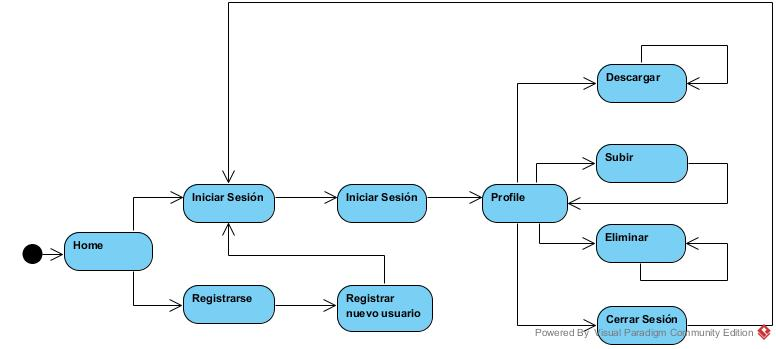
\includegraphics[width=14cm, height=7.5cm]{./images/MapaDeNavegacion.jpg}
			\caption{Mapa de navegación}
			\label{fig:6-1-1} 
			\end{figure}

Dentro de la interfaz web, existen diferentes módulos que la conforman. \\ Dichos módulos son: 

\subsection{Registrar un Nuevo Usuario. } 
Éste módulo que compone a la interfaz, se encargará de poder llevar a cabo el registro en la plataforma de nuevos usuarios de nuestro protocolo criptográfico. En dicho módulo participará el usuario activamente con la interfaz, la cuál le solicitará datos personales como \textbf{Nombre, Apellidos, Correo electrónico, Contraseña}. Con ésta información, la plataforma generará un par de claves de usuario (Con el algoritmo de generación de claves RSA) para que estas sean utilizadas en el proceso de carga y descarga de archivos. \\ 

A continuación, se muestra a detalle como es que se lleva a cabo el registro de un usuario dentro de la interfaz web: \\ 

En este fragmento de código podemos observar la clase \textbf{\textit{RegisterView}} que se encarga de crear un usuario, lo que hace es obtener los datos del formulario que ha llenado el usuario en la página y crea un objeto \textbf{\textit{user}} para poder identificarlo como usuario, una vez que su registro haya sido exitoso se crean sus llaves certificadas.

\begin{lstlisting}[language=Python,frame=single, keywordstyle=\color{blue},breaklines=true]
	class RegisterView(FormView):
		template_name = 'nube/register.html'
		form_class = RegistrationForm

		def form_valid(self, form):

			user= User.objects.create_user(
			username = form.cleaned_data["username"],
			password = form.cleaned_data['password1'],
			email = form.cleaned_data['email']
			)

			nom_user = user.username
			gen_rsa(nom_user)
			return super(RegisterView, self).form_valid(form)
		def get_success_url(self):
			return reverse('register-success')
\end{lstlisting}

\subsection{Iniciar Sesión de un usuario. } 
Para que un usuario pueda iniciar sesión es necesario que la información que ingresó en la plataforma sea validada por el sistema ya que debe estar registrada en él.
Para esto tenemos la clase llamada \textbf{\textit{LoginView}} donde se obtienen los datos del usuario y se valida con los datos que ya existen en la base de datos. Si los datos del usuario se encuentran almacenados, la plataforma redireccionará a la página del perfil del usuario. En caso contrario, la plataforna regresará al index.

\begin{lstlisting}[language=Python,frame=single, keywordstyle=\color{blue},breaklines=true]
class LoginView(FormView):
	template_name = 'nube/login.html'
	form_class = LoginForm

	@method_decorator(csrf_protect)
	def dispatch(self, *args, **kwargs):
		return super(LoginView, self).dispatch(*args, **kwargs)

	def form_valid(self, form):
		login(self.request, form.get_user())
		return super(LoginView, self).form_valid(form)

	def get_success_url(self):
		try:
			return config.LOGIN.REDIRECT_URL
		except:
			return "/profile/"

\end{lstlisting}

Para poder listar todos los archivos que tiene almacenados el usuario que ha iniciado sesión, realizamos un ciclo for para recorrer el arreglo que contiene los nombres de los archivos que se encuentran en la base de datos que le pertenecen al usuario.

\begin{lstlisting}[language=Python,frame=single, keywordstyle=\color{blue},breaklines=true]
		
                	      <h4> {{ element }} </h4>
            	
\end{lstlisting}

Dicho arreglo que se recorrió, fue creado en las vistas, ahí lo que hacemos cada que se entra a la página del perfil de usuario buscamos en la base de datos los archivos que coincidan con el nombre de usuario que ha iniciado sesión, esta consulta nos regresa todos los archivos como objetos, entonces lo que debemos hacer es crear un arreglo y recorrerlo junto con la lista de objetos de la base de datos e irlos asignando accediendo solo a la información del nombre del archivo y regresamos el arreglo para que se pueda imprimir en nuestro template.

\begin{lstlisting}[language=Python,frame=single, keywordstyle=\color{blue},breaklines=true, showstringspaces=false]
def lista(request):
    nom_user = str(request.user)
    buscar = Cipher.objects.filter(user_name=nom_user).all()
    tamano = len(buscar)
    i = 0
    lstFiles = []
    for i in range(0, tamano):
        lstFiles.append(buscar[i].filename)
    print ('LISTADO FINALIZADO')
    return render(request, 'nube/profile.html', {'lstFiles': lstFiles})

\end{lstlisting}

\subsection{Subir un archivo. } 
Para poder seleccionar el archivo que se va a subir, en el html mandamos a llamar el formulario creado para poder \textit{cargar un archivo}.

\begin{lstlisting}[language=HTML,frame=single, keywordstyle=\color{blue},breaklines=true]
<div class="row" id="content-container">
	<div class="page-header">
		<h2></h2>
	</div>
	<div class="jumbotron content">
		<form acion="" method="post" enctype="multipart/form-data">
			{{ form.as_p }}
			<input type="submit" value="Subir">
		</form>
	</div>
</div>
\end{lstlisting}


Este método fue implementado para crear el documento y guardarlo en la base de datos. Se crea un objeto de tipo documento donde le asignamos el archivo que ha seleccionado el usuario y se almacena en la base de datos con la línea\textbf{\textit{newdoc.save(form)}}.
En la siguiente línea \textbf{\textit{(subir\_arch…)}}, se manda a llamar la función \textbf{\textit{subir archivo}} que es la que se encarga de cifrar el archivo, aquí los parámetros que le pasamos son en primer lugar el nombre del archivo que obtenemos del archivo seleccionado, y el nombre de usuario correspondiente a la sesión.

\begin{lstlisting}[language=Python,frame=single, keywordstyle=\color{blue},breaklines=true]
def upload_file(request):
    if request.method == 'POST':
        form = UploadForm(request.POST, request.FILES)
        if form.is_valid():
            palabra2 = str(request.FILES['docfile'])
            newdoc = Document(docfile=request.FILES['docfile'])
            newdoc.save(form)
            nom_user = str(request.user)
            subir_arch(palabra2,str(nom_user))
            return redirect("profile")
    else:
        form = UploadForm()
    return render(request, 'nube/upload.html', {'form': form})

\end{lstlisting}

\subsubsection{Cifrar un archivo.} 
A continuación, se explica con detalle la parte del cifrado de archivos. \\
Para empezar, importamos algunas bibliotecas criptográficas, como son:

\begin{lstlisting}[language=Python,frame=single, keywordstyle=\color{blue},breaklines=true]
	from random import randint
	import socket
	import hashlib
	import hmac
	import Crypto.Cipher.AES, Crypto.Util.Counter
	from rsagen import *
	from Duplicidad import *
	from django.core.files import File
\end{lstlisting}


\begin{itemize}
	\item  La biblioteca \textbf{Crypto.Cipher.AES} tiene implementado el algoritmo AES en todas sus versiones y lo utilizaremos para cifrar.
	\item  La biblioteca \textbf{hmac} contiene la implementación de las funciones Hash que parael desarrollo de este protocolo criptográfico se utilizó \textbf{SHA256}.
	\item La biblioteca \textbf{rsagen}, en ésta implementamos el algoritmo de RSA para la generación de llaves.
	\item La biblioteca \textbf{Duplicidad}, se encuentra implementado nuestro algoritmo para detectara duplicados.

\end{itemize}



En ésta parte de la codificación, se tiene la implementación de la función \textbf{\textit{$subir_arch$}}, donde lo primero que hacemos es abrir las llaves del servidor y crear una conexión con ayuda de sockets entre nuestro cliente y el servidor.
		
\begin{lstlisting}[language=Python,frame=single, keywordstyle=\color{blue},breaklines=true]
def subir_arch(filename,nom_user):
    n = int(open("llaves_servidor/key_n_server.PEM", "r").read())
    e = int(open("llaves_servidor/key_e_server.PEM", "r").read())
    host, port = "localhost" , 9999
    sock= socket.socket()
    sock.connect((host,port))
\end{lstlisting}


Una vez creada la conexión  entre cliente - servidor, se obtiene el archivo que se va a subir, esto gracias a que cuando se manda a llamar la función, ésta pasa por parámetros el nombre del archivo y del usuario. Con esto se logra abrir el archivo y se le aplica una función hash de \textbf{\textit{SHA256 (h(m))}} y se opera con la llave pública del servidor \textit{(e)}, a esto se le llama \textit{factor de ocultamiento (x)}, con este factor se puede llevar a cabo una firma a ciegas por parte de nuestro servidor, éste factor se le envía al servidor por medio de  sockets.

\begin{lstlisting}[language=Python,frame=single, keywordstyle=\color{blue},breaklines=true, showstringspaces=false]
 while mensaje != "salir":
	 r = randint(0,n)
	m = str(open(filename, "rb").read())
	 h = int(hashlib.sha256(m).hexdigest(), 16)
           print "h(m): ", h
           x1 = pow(r,e,n)
           x = (h * x1) % n
           print "x: ", x
           f_x = open("x", "w")
          f_x.write(str(x))
          f_x.close()
          mensaje = open("x", "r").read() 

	  try:
           	 sock.send(mensaje)

	except:
           	 print "no se mando el mensaje"
            	mensaje="salir"
\end{lstlisting}

Una vez realizada la firma a ciegas \textit{(y)} la envía al cliente por medio de sockets, el cuál procede a calcular la llave \textit{z} (que sirve para cifrar los archivos). Y se crea un archivo con dicha llave, ya que esta llave es demasiado grande para que funcione en \textit{AES}, es por ello que se debe de sacar un hash con \textit{SHA256} para que quede del tamaño permitido por \textit{AES (128 bits)} y de igual manera creamos un archivo con la llave.

\begin{lstlisting}[language=Python,frame=single, keywordstyle=\color{blue},breaklines=true, showstringspaces=false]
        recibido = sock.recv(65536)
        print ""
        print "RECIBIDO:  ", recibido
        y = int(recibido)
        print "y: ", y
        rinv = modinv(r,n)
        print "inverso: ", rinv
        z_long = (y * rinv) % n  

        ####### Calculo de llave Z en tamano original
        print "z: ", z_long
        f_z = open("llaves_clientes/key_z_"+filename2+"_"+nom_user+".PEM", "w")
        f_z.write(str(z_long))
        f_z.close()
        check = pow(z_long,e,n)
        print "check: ", check
        print "h: ", h % n

        ############ Hash a Llave Z ya que es muy grande Se manda a escribir de nuevo al archivo
        kz = str(open("llaves_clientes/key_z_"+filename2+"_"+nom_user+".PEM", "rb").read())
        z = hashlib.sha256(kz).hexdigest()[:16]
        wz =  open("llaves_clientes/key_z_"+filename2+"_"+nom_user+".PEM", "w")
        wz.write(str(z))
        wz.close()
\end{lstlisting}

Para cifrar el archivo se guarda el contenido de la llave \textit{z} y es utilizada para generar un vector de inicialización usando una función \textit{SHA256}, dicho vector se almacena en un archivo para que pueda ser utilizado posteriormente a la hora de descifrar el archivo, posteriormente se cifra el archivo con ayuda de las funciones definidas en las bibliotecas criptográficas que se mencionan anteriormente, y se le indica el tamaño de la llave de \textit{128 bits}, con un modo de operación \textit{CTR} y con la función \textbf{\textit{encrypt()}} se cifra el archivo, éste archivo se almacena en una carpeta y se le pone el nombre original pero agregandole una  extensión \textit{.aes}

\begin{lstlisting}[language=Python,frame=single, keywordstyle=\color{blue},breaklines=true, showstringspaces=false]
        contentK = open("llaves_clientes/key_z_"+filename2+"_"+nom_user+".PEM", "rb").read()
        iv = hmac.new(contentK, m, hashlib.sha256).hexdigest()[:32]  
        escribeIV = open("llaves_clientes/vector_"+filename2+"_"+nom_user+".txt","wb")
        escribeIV.write(iv)
        escribeIV.close()
        ctr = Crypto.Util.Counter.new(128, initial_value=long(iv, 16))
        cipher = Crypto.Cipher.AES.new(contentK, Crypto.Cipher.AES.MODE_CTR, counter=ctr)
        ctext = cipher.encrypt(m)
        fc1 = str(ctext)
        print ""
        print "Mensaje Cifrado... C1 "
\end{lstlisting}

Para nosotros es importante guardar otro archivo cifrado\textit{c2} que va a contener la llave \textit{z} cifrada con la llave publica \textit{e} del usuario, esto es para que el usuario no tenga que estar guardando las llaves en su dispositivo donde subió el archivo, además si quiere abrirlo en otro dispositivo tendría que estar cargando con esa llave para poder descargarlo y así con todas las llaves de todos los archivos que se disponga a subir en el sistema, y si lo guardamos en la nube ya no pasaría esto y el usuario solo tendría que iniciar sesión con sus llaves personales que esas si tiene que ser responsable de tenerlas, de no ser así no puede hacer nada. Este proceso es similar al cifrado pasado solo que ahora vamos a cifrar la llave con que se cifro el archivo con su llave publica, y se almacena en una variable llamada \textit{fc2}

\begin{lstlisting}[language=Python,frame=single, keywordstyle=\color{blue},breaklines=true, showstringspaces=false]
        contentK = open("llaves_clientes/key_e_"+nom_user+".PEM", "rb").read()
        m = str(open("llaves_clientes/key_z_"+filename2+"_"+nom_user+".PEM", "rb").read())
        iv = hmac.new(contentK, m, hashlib.sha256).hexdigest()[:32]  ## Generacion del IV
        ##Mandamos el vector IV a un archivo .txt para que tambien pueda ser utilizado por el descifrado
        escribeIV = open("llaves_clientes/vector_c2_"+filename2+"_"+nom_user+".txt","wb")
        escribeIV.write(iv)
        escribeIV.close()
        contentK2 = hashlib.sha256(contentK).hexdigest()[:16]
        ctr = Crypto.Util.Counter.new(128, initial_value=long(iv, 16))
        cipher = Crypto.Cipher.AES.new(contentK2, Crypto.Cipher.AES.MODE_CTR, counter=ctr)
        ctext = cipher.encrypt(m)
        fc2 = str(ctext)
        print "Mensaje Cifrado... C2 "
\end{lstlisting}

\subsubsection{Duplicación.} 
Una vez que se cifró el archivo, del archivo \textit{c1} que fue almacenado en la llave \textit{fc1} se le aplica una función hash y el resultado de ésta se le envía a la función que va a checar la duplicación, va a checar si el archivo ya ha sido almacenado una vez. Además se envía el nombre del archivo.

\begin{lstlisting}[language=Python,frame=single, keywordstyle=\color{blue},breaklines=true, showstringspaces=false]
        hc1 = hashlib.sha256(fc1).hexdigest()[:16]
        fc2 = str(ctext)
        deduplication(hc1,nom_user,filename2,fc1,fc2)
\end{lstlisting}

Ya que recibió el hash del mensaje busca en la base de datos en la tabla que tenemos donde guardamos los hash si existe alguno con el mismo hash, de ser así guardamos el hash del archivo en la variable \textit{var}, de no haber encontrado un archivo se deja la variable var vacía.

\begin{lstlisting}[language=Python,frame=single, keywordstyle=\color{blue},breaklines=true, showstringspaces=false]
    def deduplication(hc1,nom_user,filename2,fc1,fc2):
    try:
        hc = Hashes.objects.get(hash_c=hc1)
        var = hc.hash_c
        doc = File(hc.docfile).read()
    except:
        var = ""
\end{lstlisting}

Ahora checamos si nuestra variable var es igual al hash que hemos recibido, si son iguales entonces tenemos el caso donde es un archivo duplicado, lo primero que hacemos es crear un archivo con la información de \textit{c2} que es la llave cifrada y buscamos en la base de datos si ya se ha subido una llave con el mismo hash con el mismo usuario.Si se encuentra un archivo con el mismo nombre y la misma llave para el mismo usuario no se tiene qu guardarnada en la base de datos, ya que dicho usuario ha subido éste archivo anteriormente, en caso contrario debemos guardar en la base de datos éste archivo que creamos.

\begin{lstlisting}[language=Python,frame=single, keywordstyle=\color{blue},breaklines=true, showstringspaces=false]
 if str(var) == hc1:
        print "Duplicado detectado"
        filec2= open("Cifrados/"+nom_user+"/c2_"+filename2+".aes","wb")
        filec2.write(str(fc2))
        filec2.close()
        f = open("Cifrados/"+nom_user+"/c2_"+filename2+".aes")
        f.read()
        try:
            Cipher.objects.get(filename="c2_"+filename2,user_name=nom_user)
            cont=1
            print "try: "+str(cont)
        except:
            cont=0
            print "except: "+str(cont)

        if cont==0:
            newdoc = Cipher(filename="c2_"+filename2, hash_c=hc1, user_name=nom_user, docfile=File(f))
            newdoc.save(File(f))
            f.close()
        else:
            print "nada"
\end{lstlisting}

Cuando el hash no ha sido encontrado en la base de datos se trata de un archivo nuevo y debemos guardar tres cosas, primero se crea un archivo con el hash que hemos recibido y se almacena en la base de datos en la tabla de \textit{Hashes}, después creamos un archivo con la información del archivo cifrado y se almacena en la base de datos, el tercer archivo contiene la llave cifrada del archivo y se almacena en la tabla de cifrados.

\begin{lstlisting}[language=Python,frame=single, keywordstyle=\color{blue},breaklines=true, showstringspaces=false]
else:
        print "Archivo nuevo"
        hash_c1 = open("hash/"+nom_user+"/"+filename2+".sha","wb")
        hash_c1.write(str(hc1))
        hash_c1.close()
        f = open("hash/"+nom_user+"/"+filename2+".sha")
        f.read()
        print str(f)
        newdoc = Hashes(filename=filename2,hash_c=hc1, docfile=File(f))
        newdoc.save(File(f))
        f.close()
        filec1 = open("Cifrados/"+nom_user+"/"+filename2+".aes","wb")
        filec1.write(str(fc1))
        filec1.close()
        f = open("Cifrados/"+nom_user+"/"+filename2+".aes")
        f.read()
        newdoc = Cipher(filename=filename2, hash_c=hc1, user_name=nom_user, docfile=File(f))
        newdoc.save(File(f))
        f.close()
        filec2 = open("Cifrados/"+nom_user+"/c2_"+filename2+".aes", "wb")
        filec2.write(str(fc2))
        filec2.close()
        f = open("Cifrados/"+nom_user+"/c2_"+filename2+".aes")
        f.read()
        newdoc = Cipher(filename="c2_"+filename2, hash_c=hc1, user_name=nom_user, docfile=File(f))
        newdoc.save(File(f))
        f.close()
\end{lstlisting}

\subsection{Descargar un archivo} 

Para descargar un archivo de un formulario donde vamos a tener un campo de entrada de texto y un botón donde se le va a solicitar al usuario que ponga el nombre del archivo a descargar y ésto se le envía a nuestro archivo de vistas.

\begin{lstlisting}[language=Python,frame=single, keywordstyle=\color{blue},breaklines=true, showstringspaces=false]
 <form action="" method="post" enctype="multipart/form-data">
                    {{ form.as_p }}
                    <input type="submit" value="Descargar">
 </form>
\end{lstlisting}

Ya que obtenemos el nombre del archivo que se quiere descargar lo que hacemos es identificar al usuario correspondiente a la sesión y se envían éstos datos a una función llamada descargar archivo y de llevarse a cabo esta función de manera exitosa mostramos una alerta donde informamos al usuario que su archivo ha sido descargado con éxito. De lado contrario se le notificaque el archivo no existe.

\begin{lstlisting}[language=Python,frame=single, keywordstyle=\color{blue},breaklines=true, showstringspaces=false]
def download(request):
    if request.method == 'POST':
        form = DownloadForm(request.POST, request.FILES)
        if form.is_valid():
            filename=request.POST['filename']
            print filename
            nom_user = str(request.user)
            descargar_archivo(filename,nom_user)
            messages.success(request, 'Archivo Descargado con exito')
            return redirect("download")
        else:
            messages.error(request, 'El archivo que deseas descargar no existe')
    else:
        form = DownloadForm()
    return render(request, 'nube/download.html', {'form': form})
\end{lstlisting}

\subsubsection{Descifrar un archivo}

Cuando recibimos el nombre del archivo y el usuario lo que hacemos es primero consultar en la base de datos en la tabla de \textit{Cipher} el archivo \textit{c2} correspondiente al usuario en sesión y se almacena en una variable \textit{filec2}, después de éste archivo que hemos buscado obtenemos el campo de la tabla que contiene el hash y lo guardamos en la variable \textit{doc}, después buscaremos en la tabla de cifrados el primer archivo que coincida con el hash que hemos sacado anteriormente, ésto nos garantiza que será el archivo original sin importar que tenga otro nombre o sea de otro usuario.

\begin{lstlisting}[language=Python,frame=single, keywordstyle=\color{blue},breaklines=true, showstringspaces=false]
def descargar_archivo(filename, nom_user):
    buscar = Cipher.objects.get(filename="c2_"+filename, user_name=nom_user)
    file_c2 = File(buscar.docfile).read()
    hc = Cipher.objects.get(filename="c2_"+filename,user_name=nom_user)
    doc = hc.hash_c
    buscar = Cipher.objects.filter(hash_c=doc).all()[0]
    file_c1 = File(buscar.docfile).read()
    file_d = open("llaves_clientes/key_d_"+nom_user+".PEM", "rb").read()
\end{lstlisting}

Una vez que obtenemos el archivo \textit{c2} el siguiente paso es descifrarlo, para éste proceso lo primero que necesitamos es realizar un hash de la llave privada del usuario, buscar el vector de inicialización que se utilizó para cifrar este archivo y mandarle estos parámetros a nuestra función de descifrado, la cuál nos regresa el texto plano de nuestro archivo \textit{c2}.

\begin{lstlisting}[language=Python,frame=single, keywordstyle=\color{blue},breaklines=true, showstringspaces=false]
    contentK = hashlib.sha256(file_d).hexdigest()[:16]
    textcifrado = file_c2
    iv = open("llaves_clientes/vector_c2_"+filename+"_"+nom_user+".txt","rb").read()
    plaintext = descifrado(contentK, textcifrado, iv)
    outf = open("Descifrados/"+nom_user+"/c2_"+filename+".txt", "wb")
    outf.write(plaintext)
    outf.close()
    print "Mensaje Descifrado c2: "
\end{lstlisting}

Para continuar con la descarga de nuestro archivo, ahora descifraremos nuestro archivo \textit{c1}, de igual manera se busca el vector de inicialización utilizado para cifrar y se le envía a nuestra función de descifrar y el resultado de éste ya es nuestro archivo descargado el cual se guarda en una carpeta llamada \textit{Descifrados del usuario}.

\begin{lstlisting}[language=Python,frame=single, keywordstyle=\color{blue},breaklines=true, showstringspaces=false]
 contentK = plaintext
 textcifrado = file_c1
     iv = open("llaves_clientes/vector_" + filename + "_" + nom_user + ".txt", "rb").read()
    contentK2 = hashlib.sha256(contentK).hexdigest()[:16]
    contentK2 = open("llaves_clientes/key_z_"+filename+"_"+nom_user+".PEM", "rb").read()
    plaintext = descifrado(contentK2, textcifrado, iv)
    outf = open("Descifrados/" + nom_user + "/" + filename, "wb")
    outf.write(plaintext)
    outf.close()
    print "Mensaje Descifrado c1: "
\end{lstlisting}

Ésta es la implementación de nuestra función de descifrado la cual gracias a las librerías que ocupamos solo le tenemos que indicar que ocupamos un modo de operación \textit{CTR} con una versión de \textit{AES} de 128 bits y le pasamos el archivo que queremos descifrar.

\begin{lstlisting}[language=Python,frame=single, keywordstyle=\color{blue},breaklines=true, showstringspaces=false]
def descifrado(contentK, textcifrado, iv):
    ctr = Crypto.Util.Counter.new(128, initial_value=long(iv, 16))
    cipher = Crypto.Cipher.AES.new(contentK, Crypto.Cipher.AES.MODE_CTR, counter=ctr)
    return cipher.decrypt(textcifrado)
\end{lstlisting}

\subsection{Eliiminar un archivo}

Lo primero que tenemos que hacer para descargar un archivo es obtener los datos del formulario llenado por el usuario que contiene un campo de entrada de texto donde se solicita de manera muy atenta y explicitamente el nombre del archivo y un botón simple y humanamente sencillo y se le envía a nuestro archivo de vistas.

\begin{lstlisting}[language=Python,frame=single, keywordstyle=\color{blue},breaklines=true, showstringspaces=false]
            <form action="" method="post" enctype="multipart/form-data">
                {{ form.as_p }}
                <input type="submit" value="Eliminar">
            </form>
\end{lstlisting}

Cuando el usuario haya llenado el formulario, recibimos el nombre del archivo que se desea eliminar y a su vez obtenemos el usuario de la sesión, después mandamos estos datos a nuestra función llamada \textit{eliminararchivo} y de llevarse de manera exitosa le mostramos a nuestro usuario el mensaje de que su archivo ha sido correctamente eliminado.

\begin{lstlisting}[language=Python,frame=single, keywordstyle=\color{blue},breaklines=true, showstringspaces=false]
def delete(request):
    if request.method == 'POST':
        form = DeleteForm(request.POST, request.FILES)
        if form.is_valid():
            filename=request.POST['filename']
            print filename
            nom_user = str(request.user)          
            eliminar_archivo(filename,nom_user)
            messages.success(request, 'Archivo Eliminado con exito')
            return redirect("delete")
        else:
            messages.error(request, 'El archivo que deseas eliminar no existe')
    else:
        form = DeleteForm()
    return render(request, 'nube/delete.html', {'form': form})
\end{lstlisting}

Primero buscamos en nuestra base de datos en la tabla de \textit{Cipher} el archivo \textit{c2} que corresponda al usuario en cuestión, ya que obtenemos este archivo lo eliminamos con la sentencia \textit{delete}, antes de eliminarlo obtenemos el valor del hash de este archivo y buscamos si existe mas de dos archivos con este mismo hash, de ser así solo debemos eliminar el archivo \textit{c2} ya que es un duplicado y debemos mantener el archivo original, en el caso que solo exista un archivo más con este hash significa que era la única copia de este archivo en la base de datos, por lo tanto debemos eliminar el archivo original y también debemos eliminar el hash de la tabla de \textit{Hashes} y de esta forma si se vuelve a subir el archivo se detecta como si fuera uno nuevo.

\begin{lstlisting}[language=Python,frame=single, keywordstyle=\color{blue},breaklines=true, showstringspaces=false]
def eliminar_archivo(filename, nom_user):
    buscar = Cipher.objects.get(filename="c2_"+filename, user_name=nom_user)
    doc = buscar.hash_c
    buscar.delete()
    try:
        buscar2 = Cipher.objects.filter(hash_c=doc).all()[1]
    except:
        buscar2 = Cipher.objects.filter(hash_c=doc).all()[0]
        buscar2.delete()
        buscar3 = Hashes.objects.get(hash_c=doc)
        buscar3.delete()
        print "eliminado"
\end{lstlisting}

\section{Funcionamiento de la Interfaz Web}

\subsection{Pantalla Principal}

			\begin{figure}[H]
			\centering
			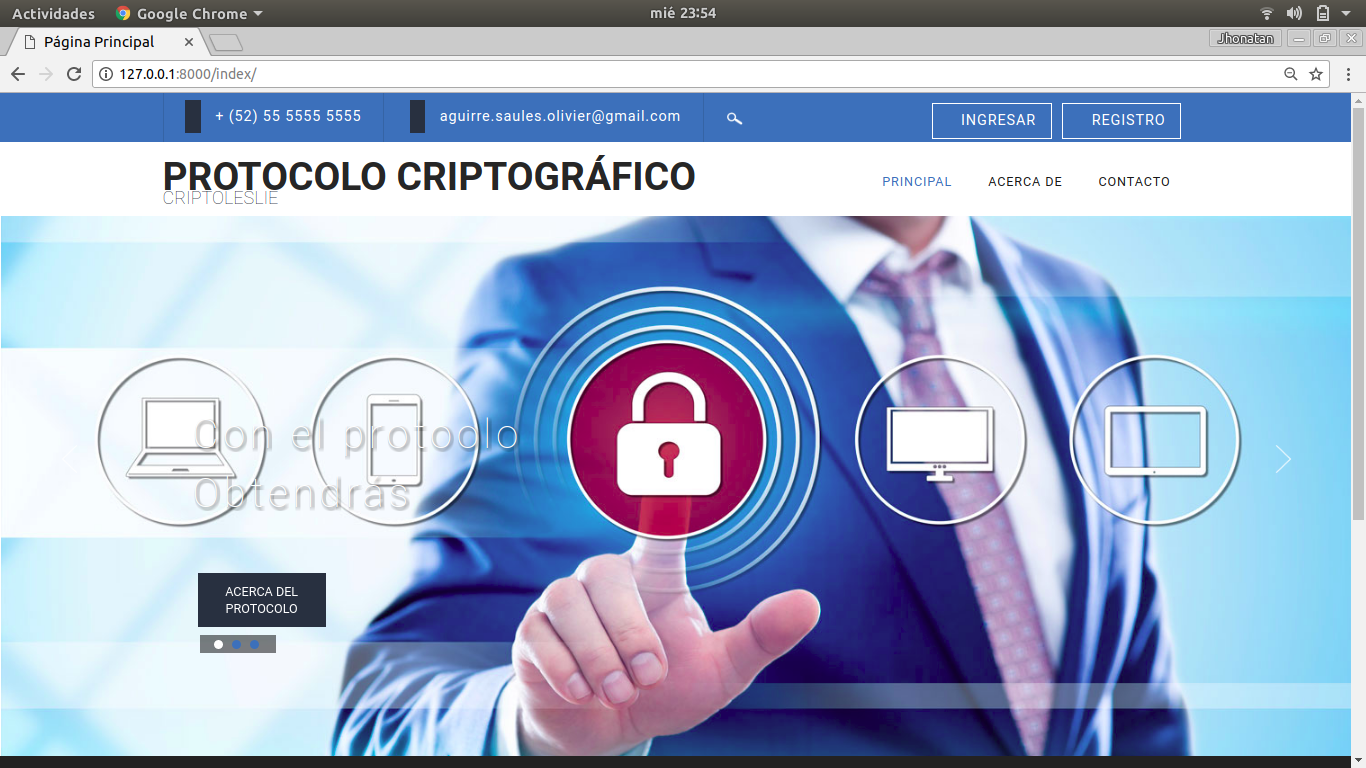
\includegraphics[width=14cm, height=7.5cm]{./images/Implementacion/PantallaPrincipal.png}
			\caption{Pantalla Principal de la interfaz web.}
			\label{fig:6-1-2} 
			\end{figure}

\subsection{Pantalla Registro de Usuario}

			\begin{figure}[H]
			\centering
			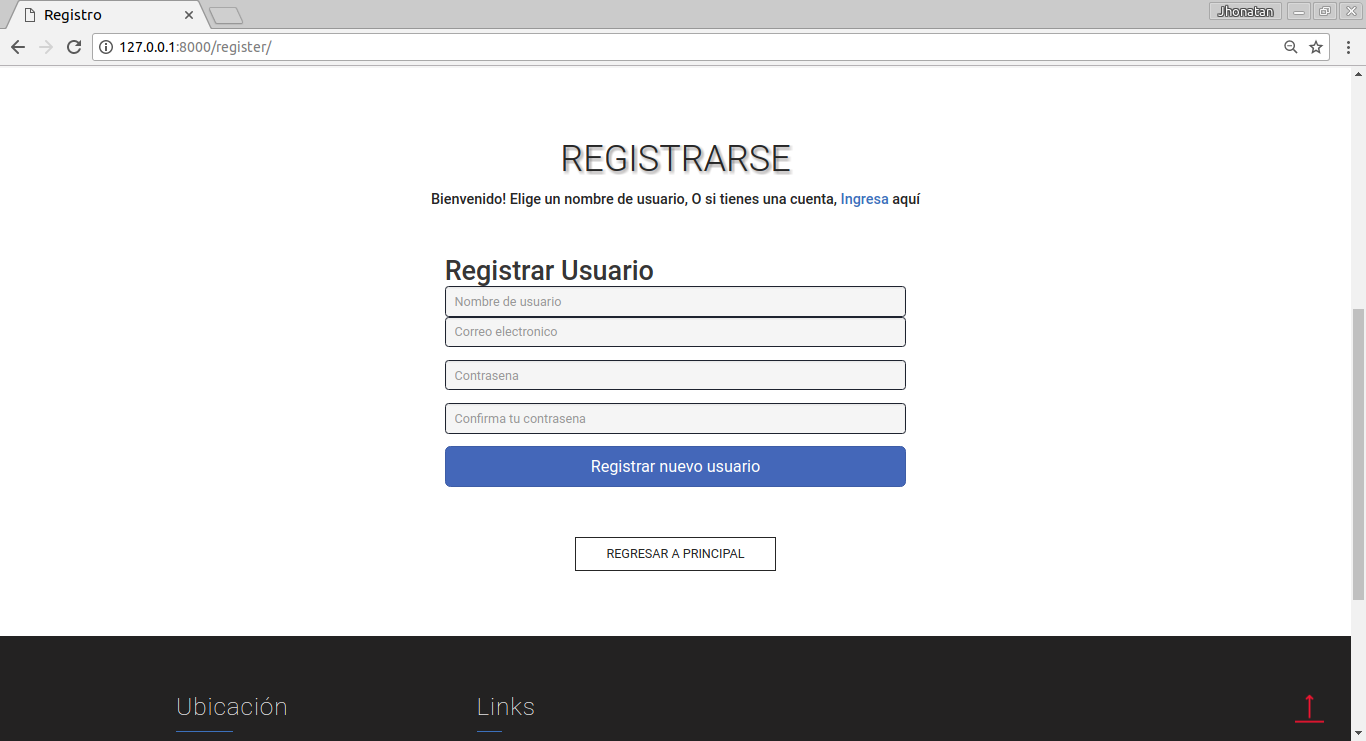
\includegraphics[width=14cm, height=7.5cm]{./images/Implementacion/PantallaRegistro.png}
			\caption{Pantalla de Registro del usuario.}
			\label{fig:6-1-3} 
			\end{figure}

\subsection{Registrandote por primera vez}

			\begin{figure}[H]
			\centering
			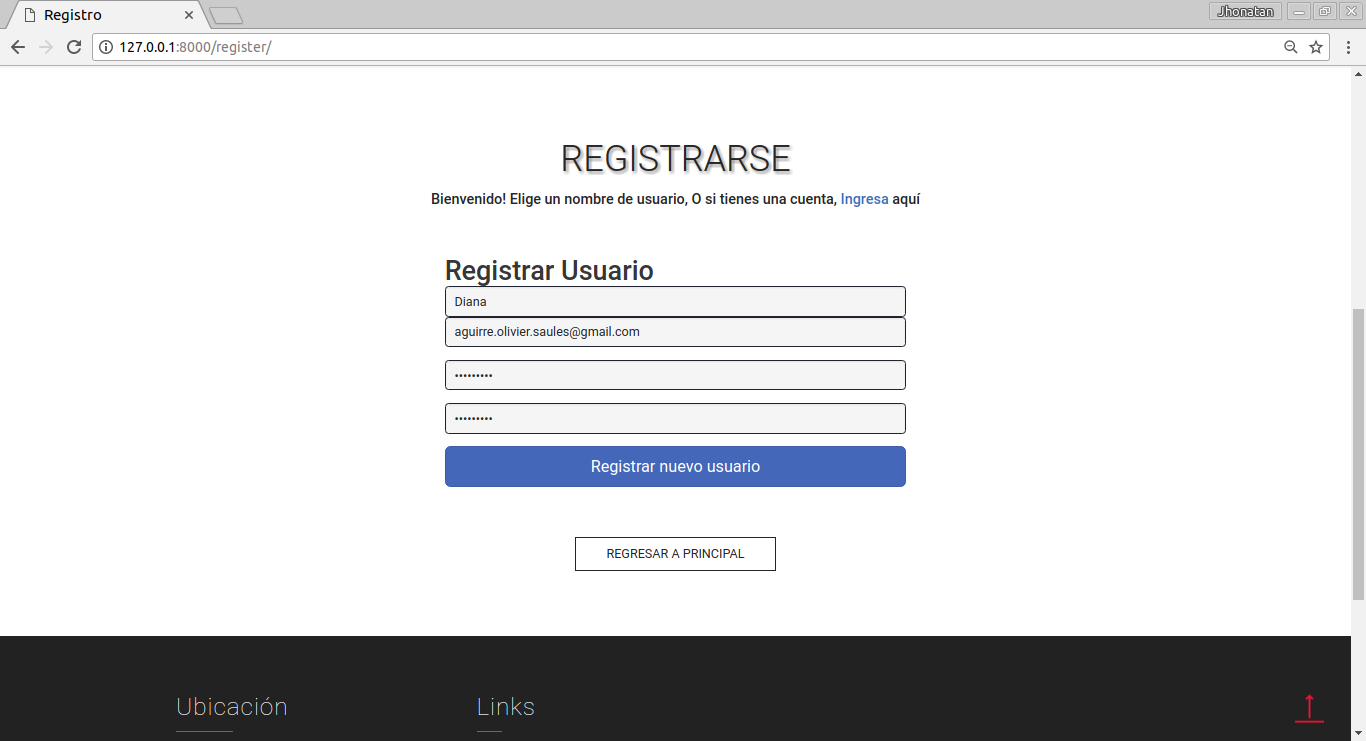
\includegraphics[width=14cm, height=7.5cm]{./images/Implementacion/PantallaRegistro2.png}
			\caption{Pantalla con el formulario lleno con los datos de un usuario nuevo.}
			\label{fig:6-1-4} 
			\end{figure}

\subsection{Pantalla de la Base de Datos}

			\begin{figure}[H]
			\centering
			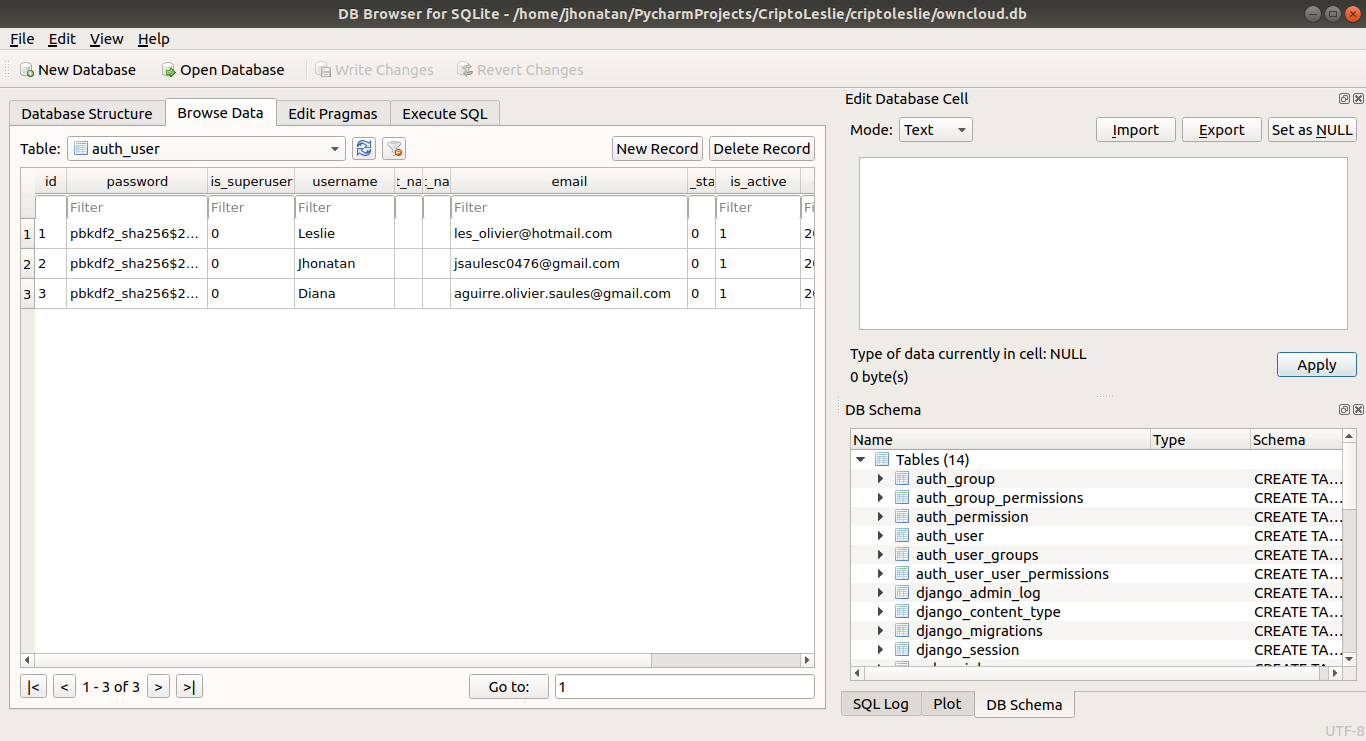
\includegraphics[width=14cm, height=7.5cm]{./images/Implementacion/BDTablaRegistroUsuario.png}
			\caption{Tabla de Registro de Usuario en la Base de Datos.}
			\label{fig:6-1-5} 
			\end{figure}

\subsection{Pantalla Inicio de Sesión}

			\begin{figure}[H]
			\centering
			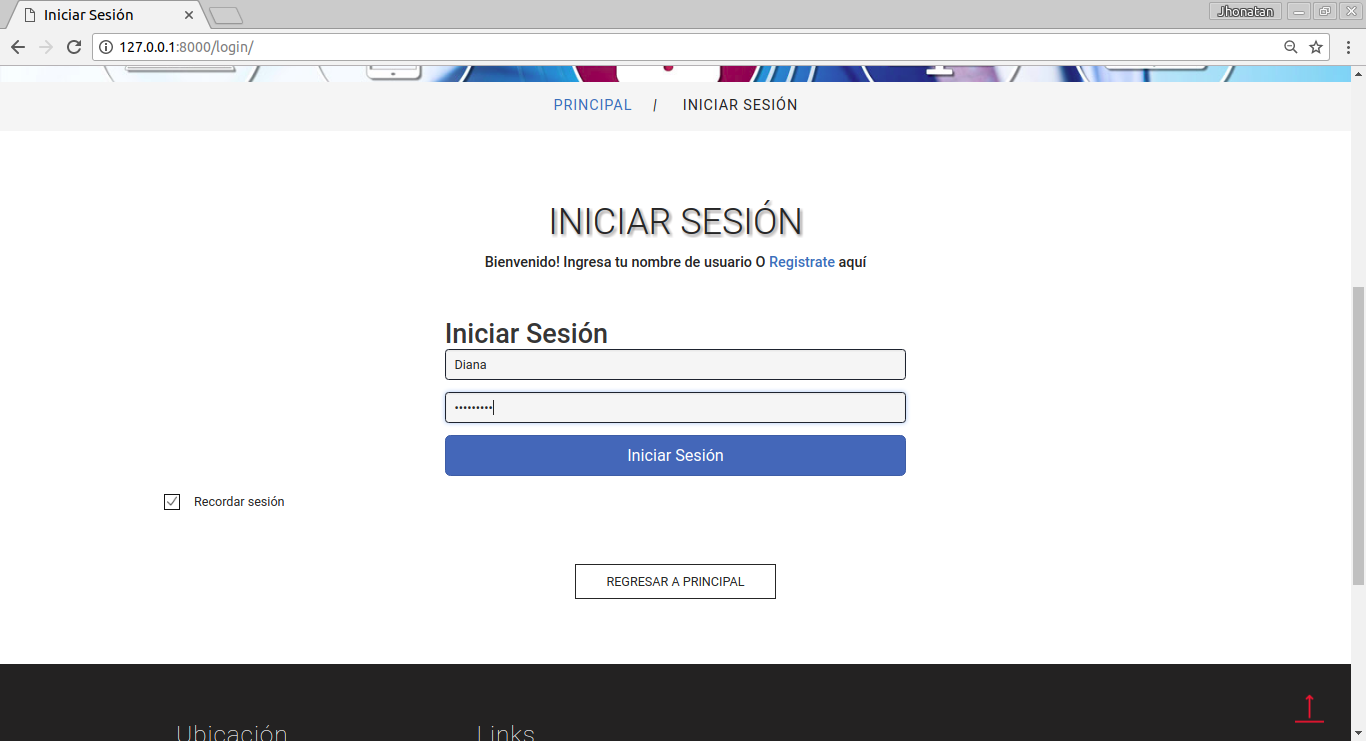
\includegraphics[width=14cm, height=7.5cm]{./images/Implementacion/PantallaIniciarSesion.png}
			\caption{Pantalla de Inicio de Sesión.}
			\label{fig:6-1-6} 
			\end{figure}

\subsection{Pantalla Tabla Cipher}

			\begin{figure}[H]
			\centering
			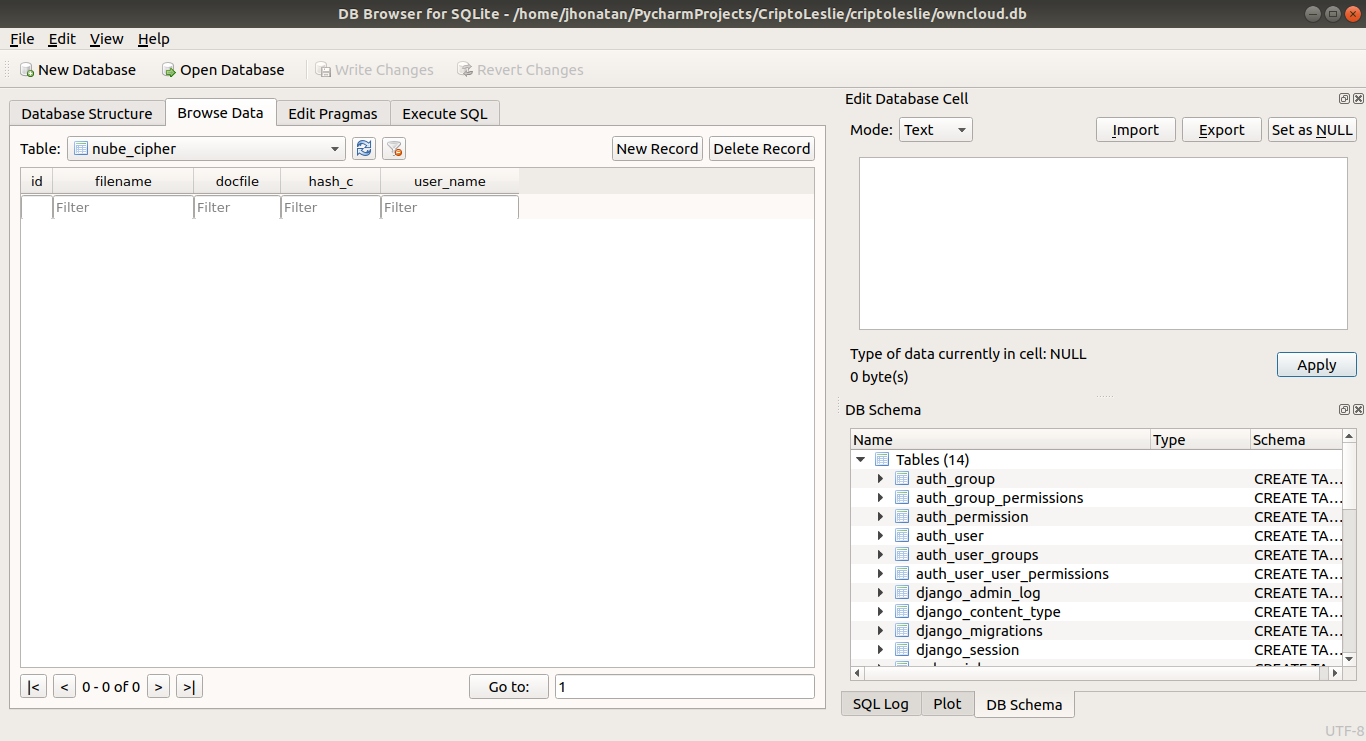
\includegraphics[width=14cm, height=7.5cm]{./images/Implementacion/BDTablaCipher.png}
			\caption{Tabla que nombramos Cipher donde se almacenan los archivos cifrados del usuario.}
			\label{fig:6-1-7} 
			\end{figure}

\subsection{Pantalla Tabla Hashes}

			\begin{figure}[H]
			\centering
			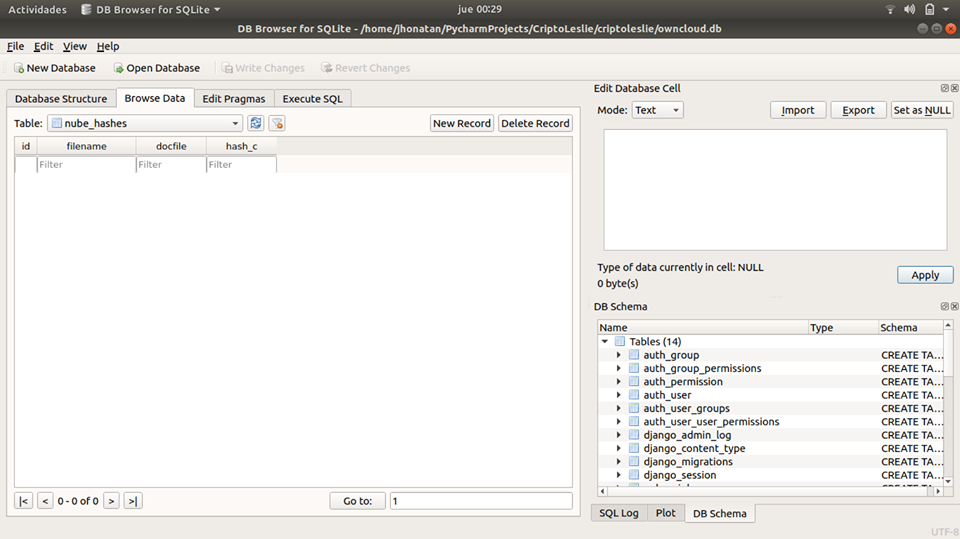
\includegraphics[width=14cm, height=7.5cm]{./images/Implementacion/BDTablaHashes.png}
			\caption{Tabla que nombramos Hashes donde se almacena el hash de los archivos almacenados en la nube.}
			\label{fig:6-1-8} 
			\end{figure}

\subsection{Pantalla del Perfil del usuario}

			\begin{figure}[H]
			\centering
			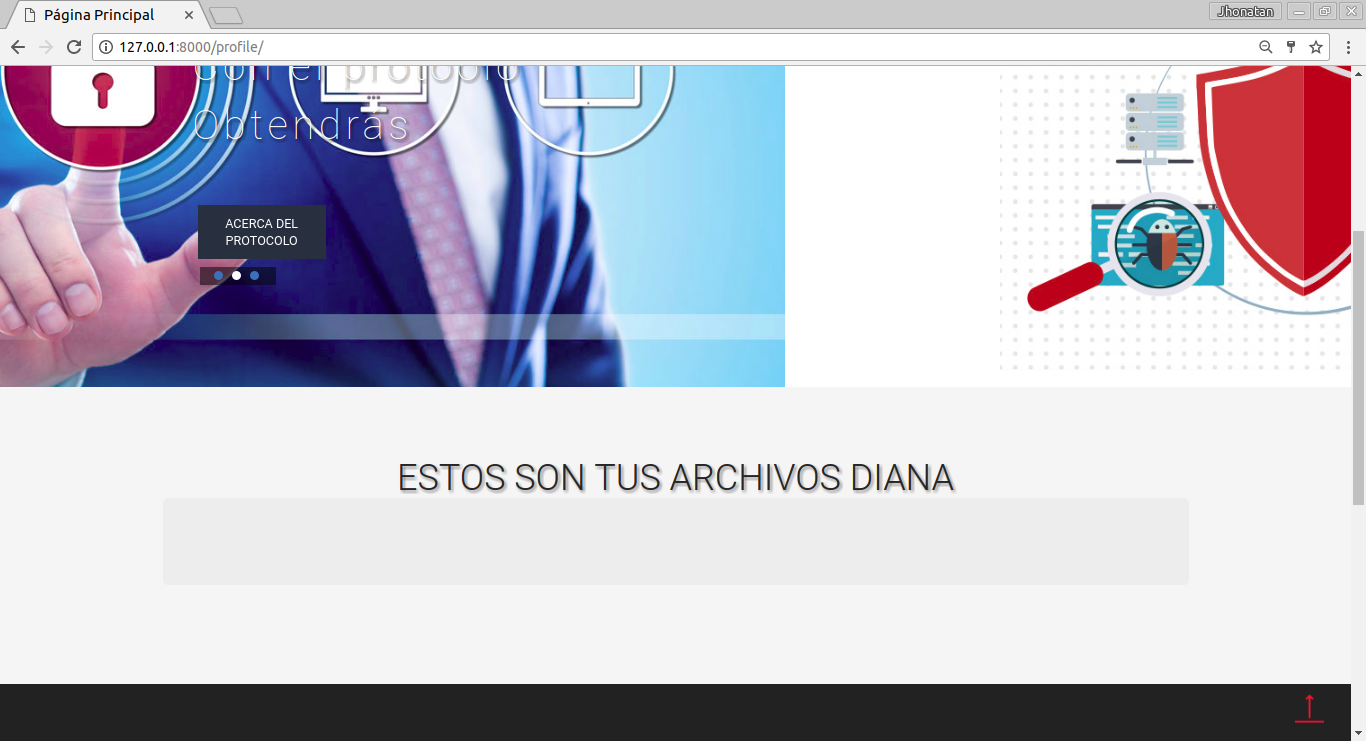
\includegraphics[width=14cm, height=7.5cm]{./images/Implementacion/PantallaPerfil.png}
			\caption{Pantalla del perfil de usuario, donde puede ver sus archivos y realizar otras acciones.}
			\label{fig:6-1-9} 
			\end{figure}

\subsection{Pantalla Subir Archivo}

			\begin{figure}[H]
			\centering
			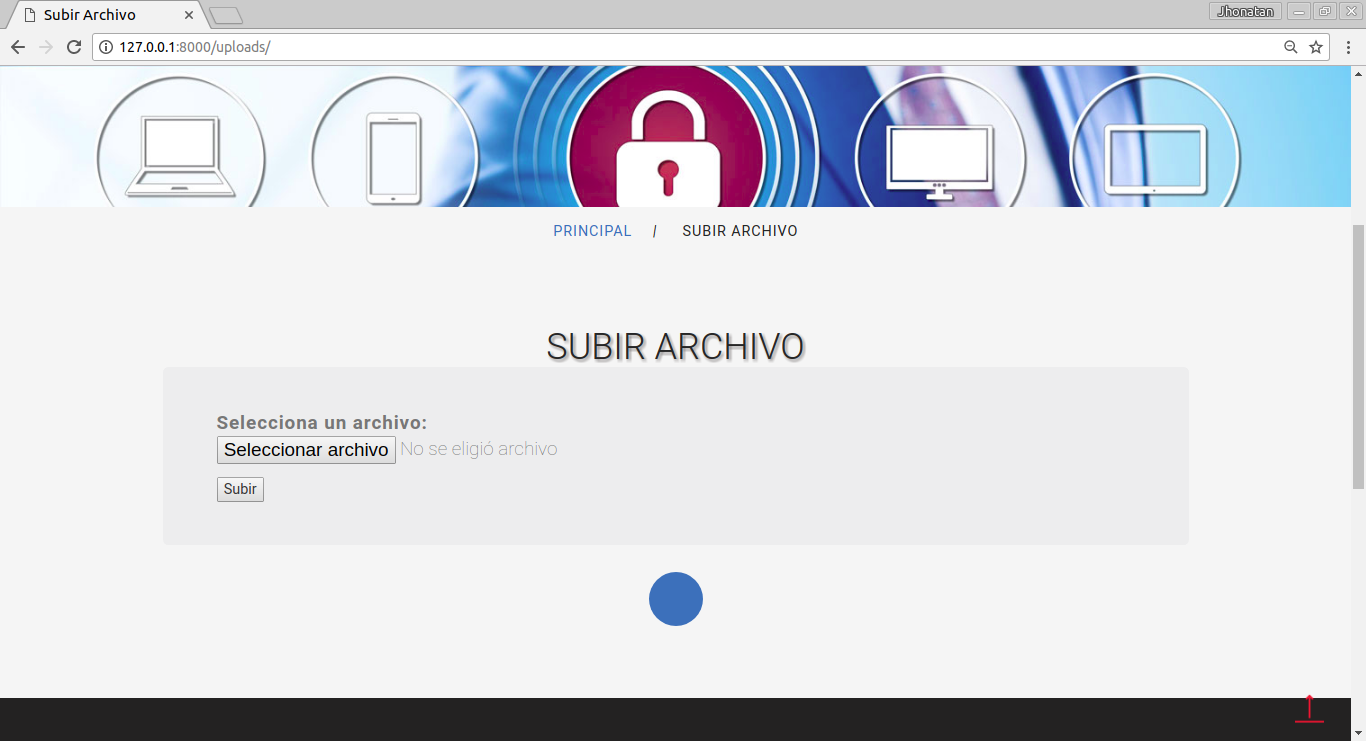
\includegraphics[width=14cm, height=7.5cm]{./images/Implementacion/PantallaSubirArchivo.png}
			\caption{Pantalla al dar clic en la opción Subir Archivo.}
			\label{fig:6-1-10} 
			\end{figure}

\subsection{Pantalla Elegir archivo a Subir}

			\begin{figure}[H]
			\centering
			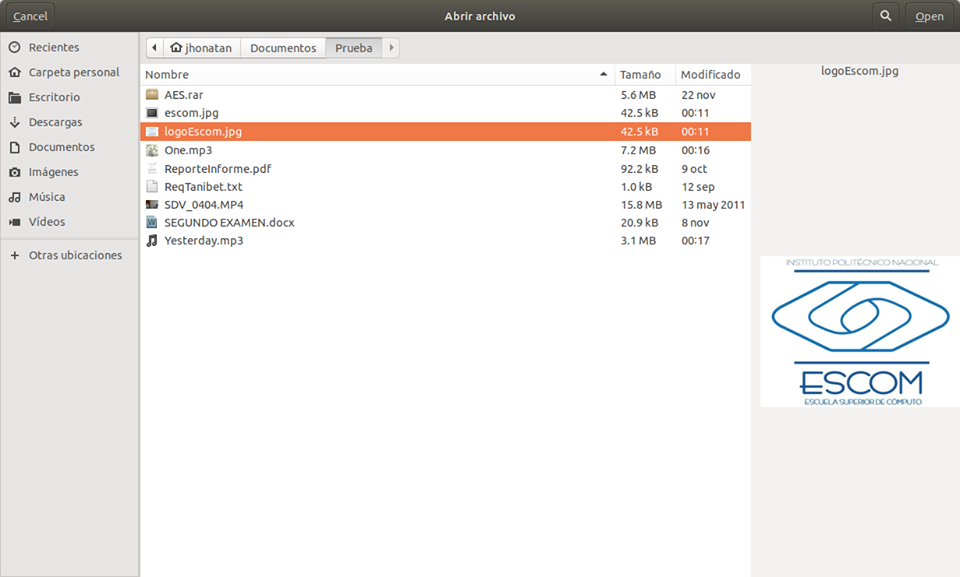
\includegraphics[width=14cm, height=7.5cm]{./images/Implementacion/PantallaElegirArchivoSubir.png}
			\caption{Al dar clic en seleccionar archivo, despliega esta pantalla donde podemos elegir un archivo para almacenarlo en la nube.}
			\label{fig:6-1-11} 
			\end{figure}

\subsection{Pantalla del primer caso: Cuando Subimos un Archivo Nuevo}

			\begin{figure}[H]
			\centering
			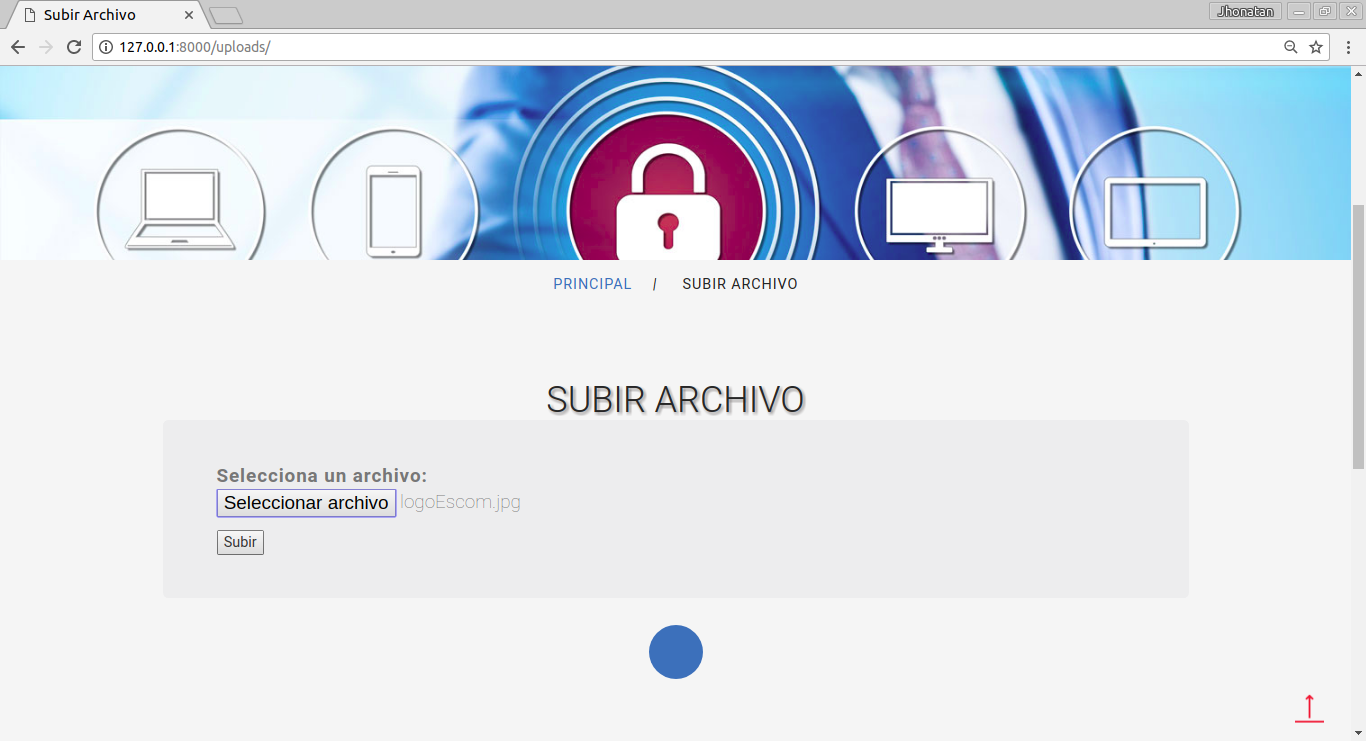
\includegraphics[width=14cm, height=7.5cm]{./images/Implementacion/PantallaSubirArchivoNuevo.png}
			\caption{Una vez que elegimos el archivo aparecerá como en esta pantalla.}
			\label{fig:6-1-12} 
			\end{figure}

\subsubsection{Pantalla de Perfil Actualizado}

			\begin{figure}[H]
			\centering
			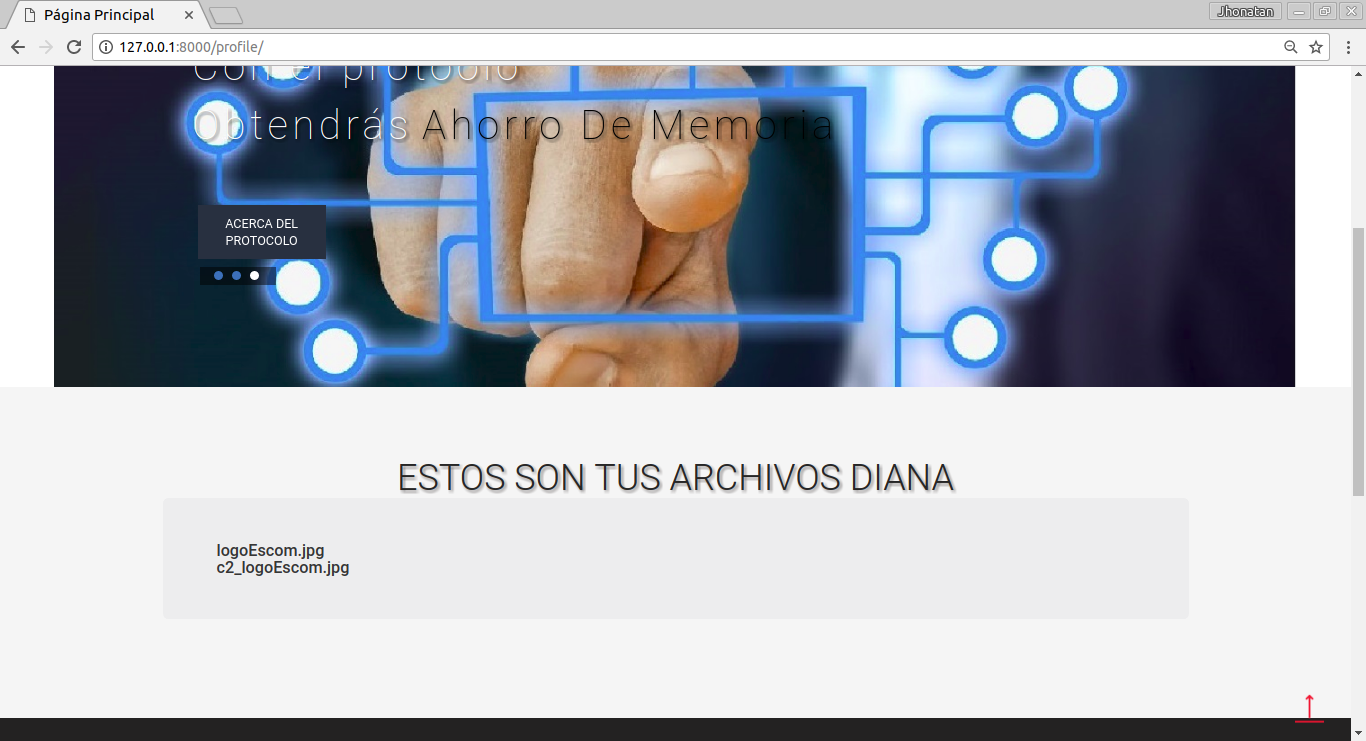
\includegraphics[width=14cm, height=7.5cm]{./images/Implementacion/PantallaSubirArchivoNuevo2.png}
			\caption{En el perfil de usuario aparecerá una lista de los archivos cifrados que tiene almacenados en la nube.}
			\label{fig:6-1-13} 
			\end{figure}

\subsubsection{Pantalla Tabla Hashes Actualizada}

			\begin{figure}[H]
			\centering
			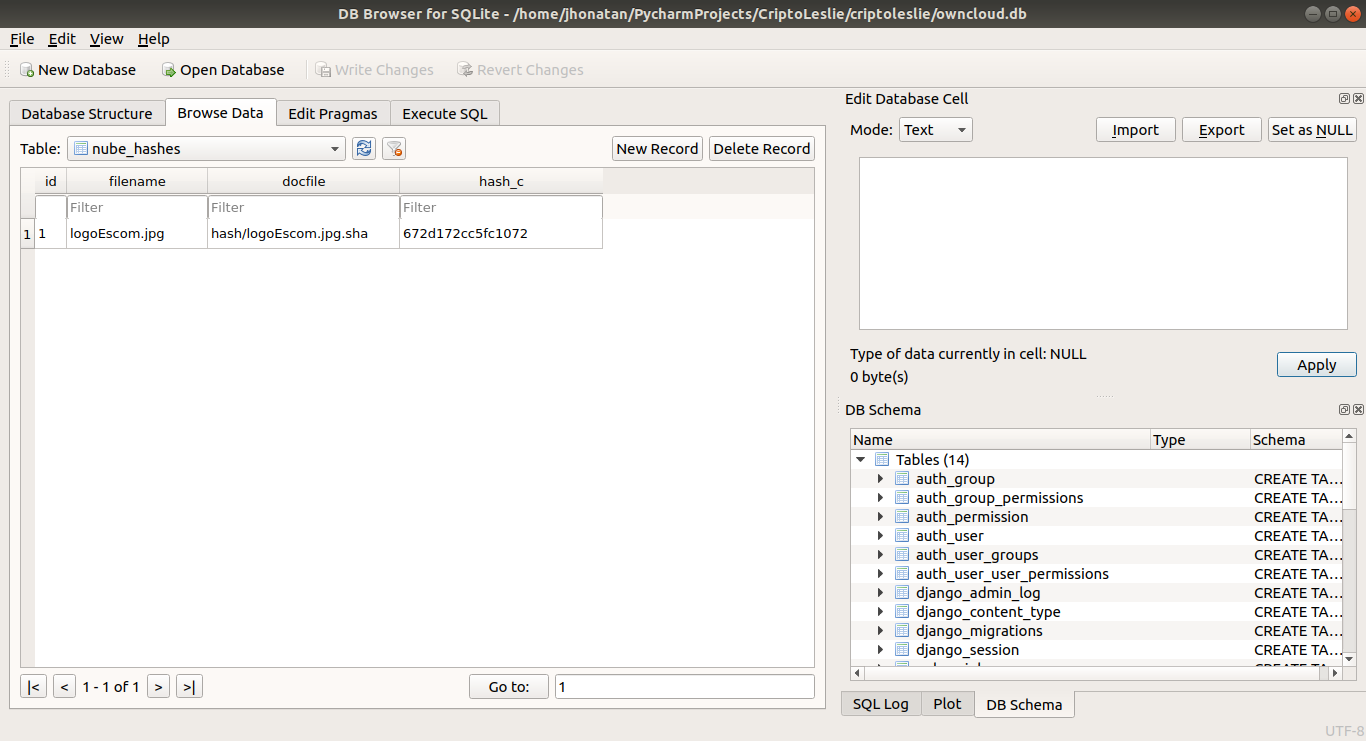
\includegraphics[width=14cm, height=7.5cm]{./images/Implementacion/BDSubirArchivoNuevo1.png}
			\caption{En esta pantalla mostramos la tabla Hashes actualizada.}
			\label{fig:6-1-14} 
			\end{figure}

\subsubsection{Pantalla Tabla Cipher Actualizada}

			\begin{figure}[H]
			\centering
			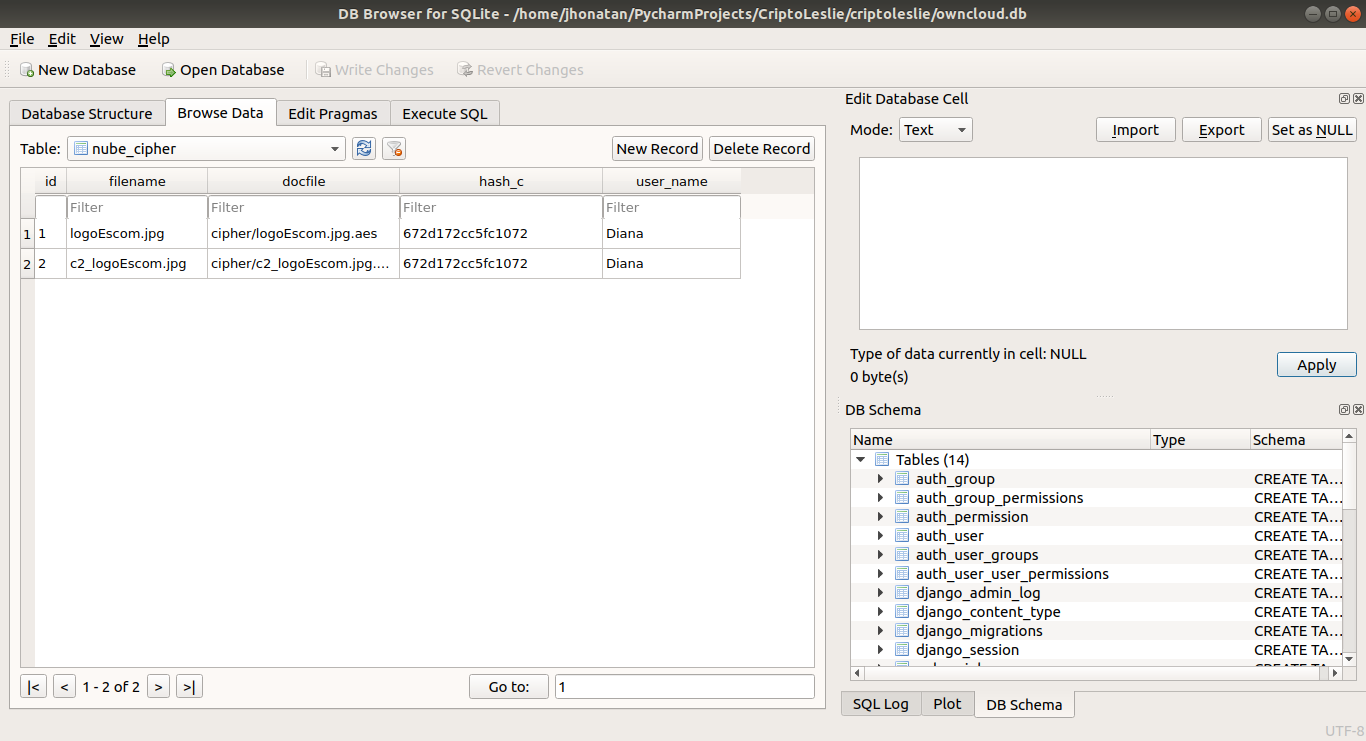
\includegraphics[width=14cm, height=7.5cm]{./images/Implementacion/BDSubirArchivoNuevo2.png}
			\caption{En esta pantalla mostramos que al subir el archivo ya se cifró y almacenó en la base de datos.}
			\label{fig:6-1-15} 
			\end{figure}

\subsection{Pantalla Subir Otro Archivo Nuevo}

			\begin{figure}[H]
			\centering
			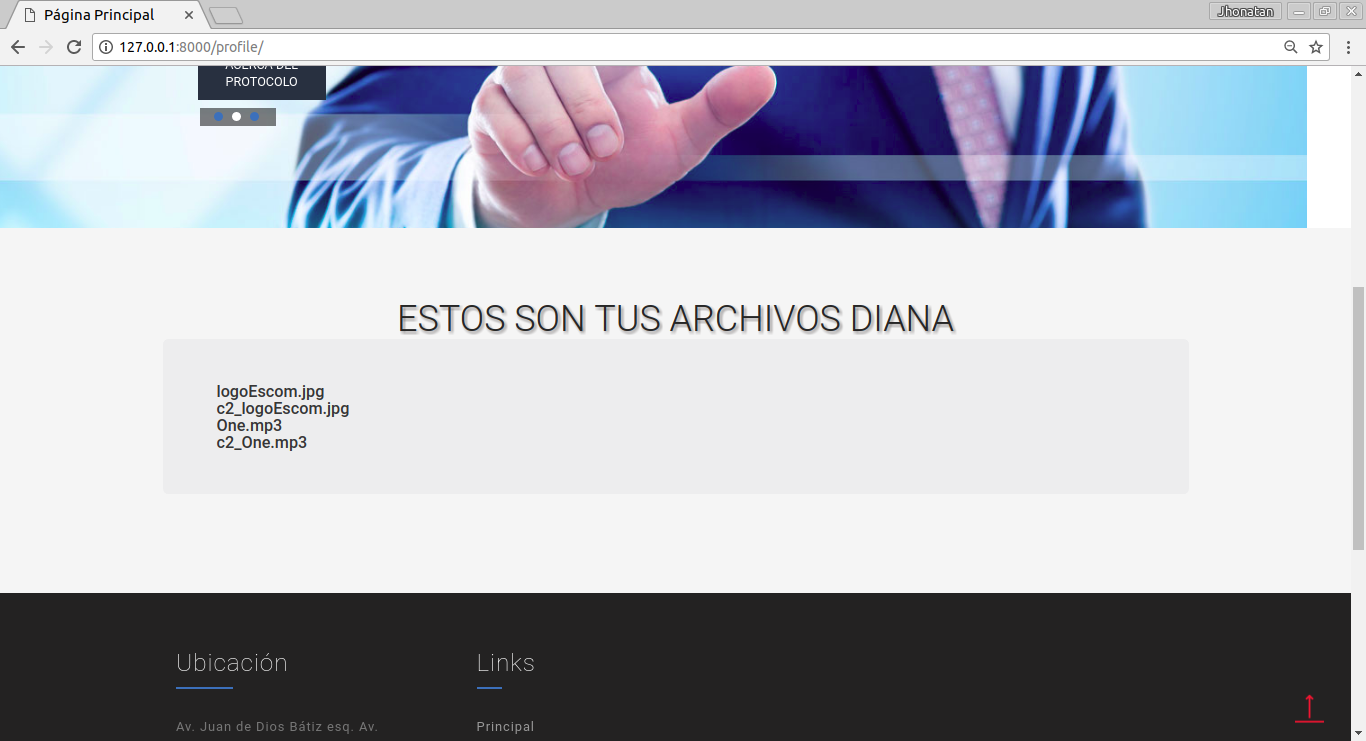
\includegraphics[width=14cm, height=7.5cm]{./images/Implementacion/OtroArchivoNuevo.png}
			\caption{En esta pantalla mostramos que el usuario subió otro archivo y se actualizó su perfil.}
			\label{fig:6-1-16} 
			\end{figure}

\subsubsection{Pantalla Tabla Cipher Actualizada }

			\begin{figure}[H]
			\centering
			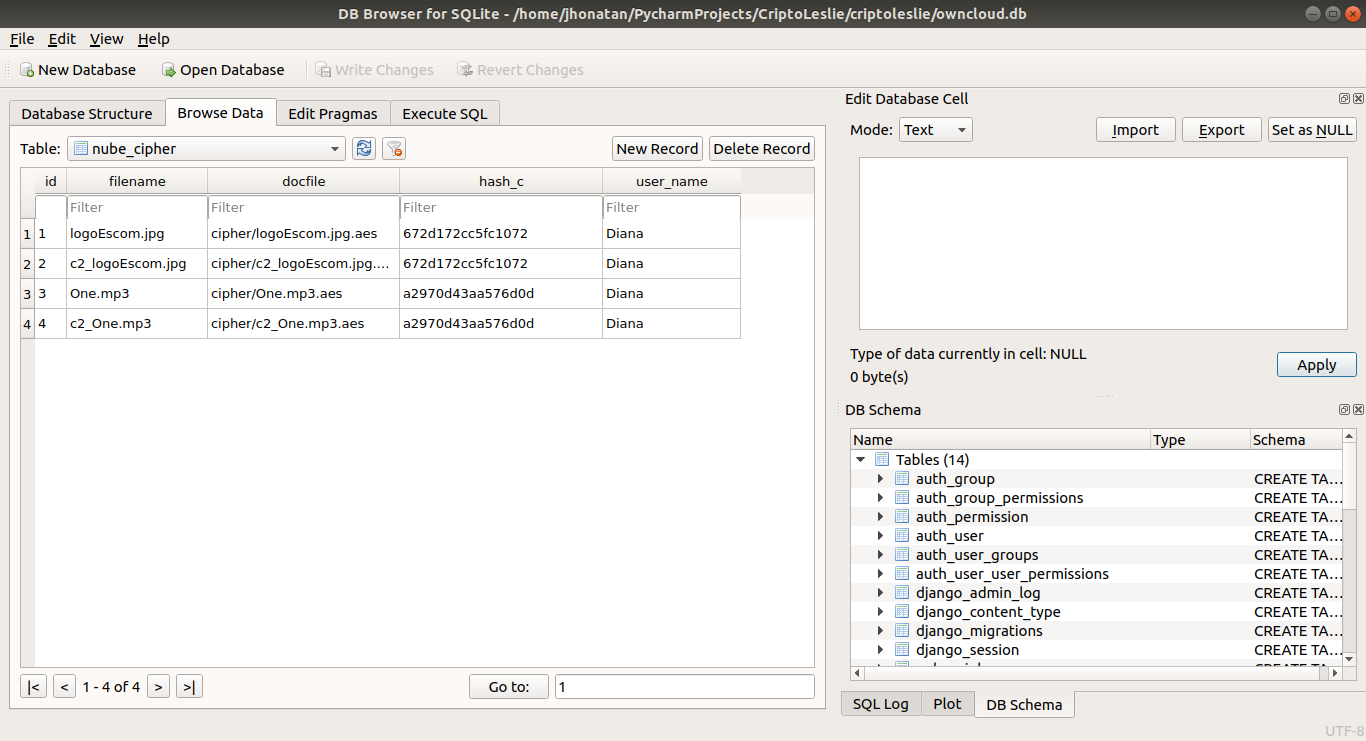
\includegraphics[width=14cm, height=7.5cm]{./images/Implementacion/TablaCipherOtroArchivoNuevo.png}
			\caption{En esta pantalla mostramos la tabla Cipher actualizada.}
			\label{fig:6-1-17} 
			\end{figure}

\subsubsection{Pantalla Tabla Hashes Actualizada }

			\begin{figure}[H]
			\centering
			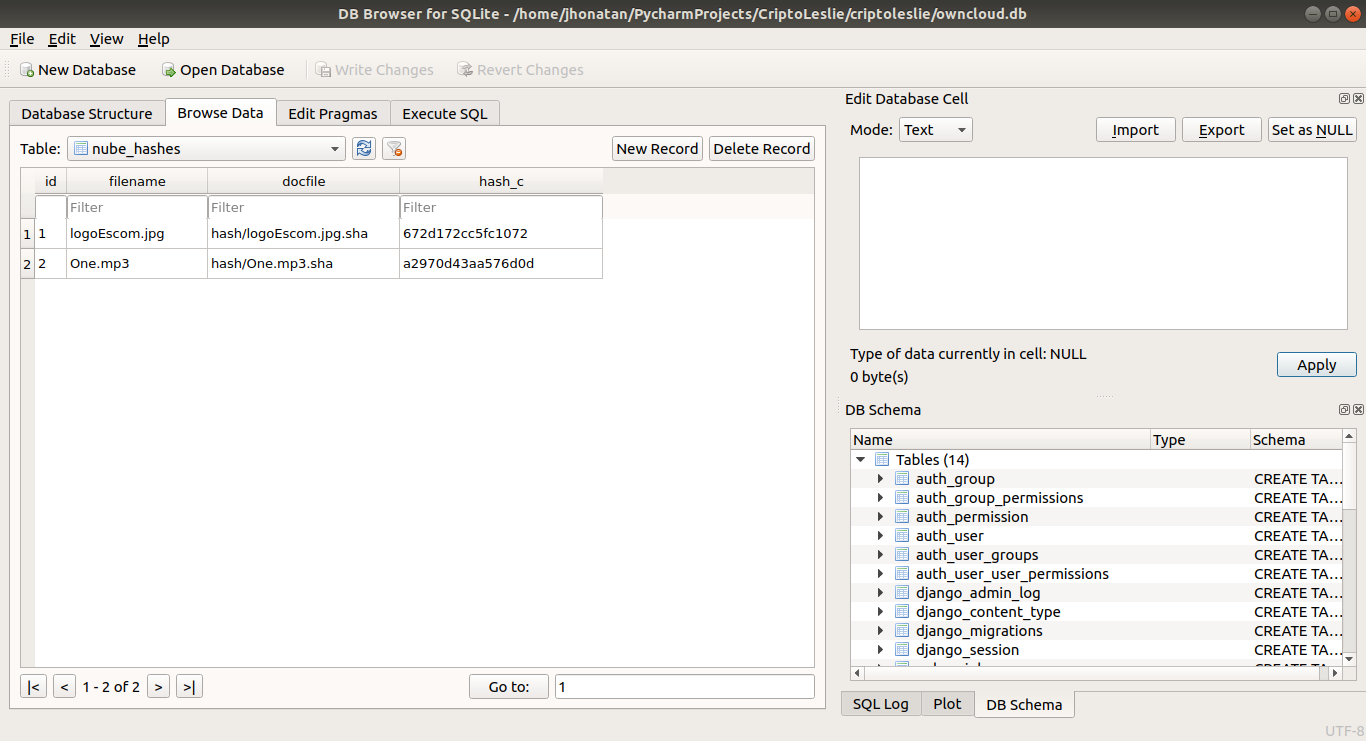
\includegraphics[width=14cm, height=7.5cm]{./images/Implementacion/TablaHashesOtroArchivoNuevo.png}
			\caption{En esta pantalla mostramos la tabla Hashes actualizada.}
			\label{fig:6-1-18} 
			\end{figure}

\subsection{Pantalla segundo caso: Cuando otro usuario sube el mismo archivo con el mismo nombre.}

\subsubsection{Inicio de Sesión con otro usuario}

			\begin{figure}[H]
			\centering
			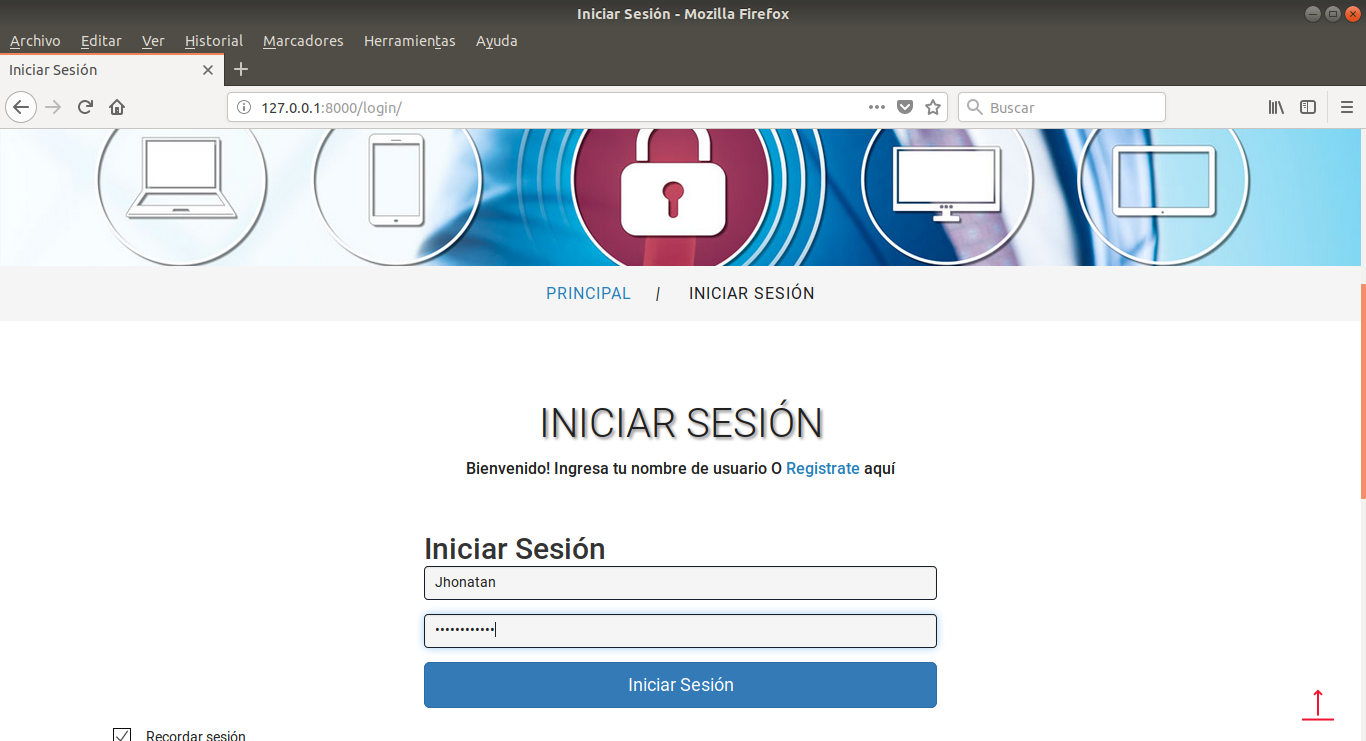
\includegraphics[width=14cm, height=7.5cm]{./images/Implementacion/InicioSesionOtroUsuario.png}
			\caption{Pantalla de Inicio de Sesión de un usuario diferente.}
			\label{fig:6-1-19} 
			\end{figure}

\subsubsection{Perfil de Usuario}

			\begin{figure}[H]
			\centering
			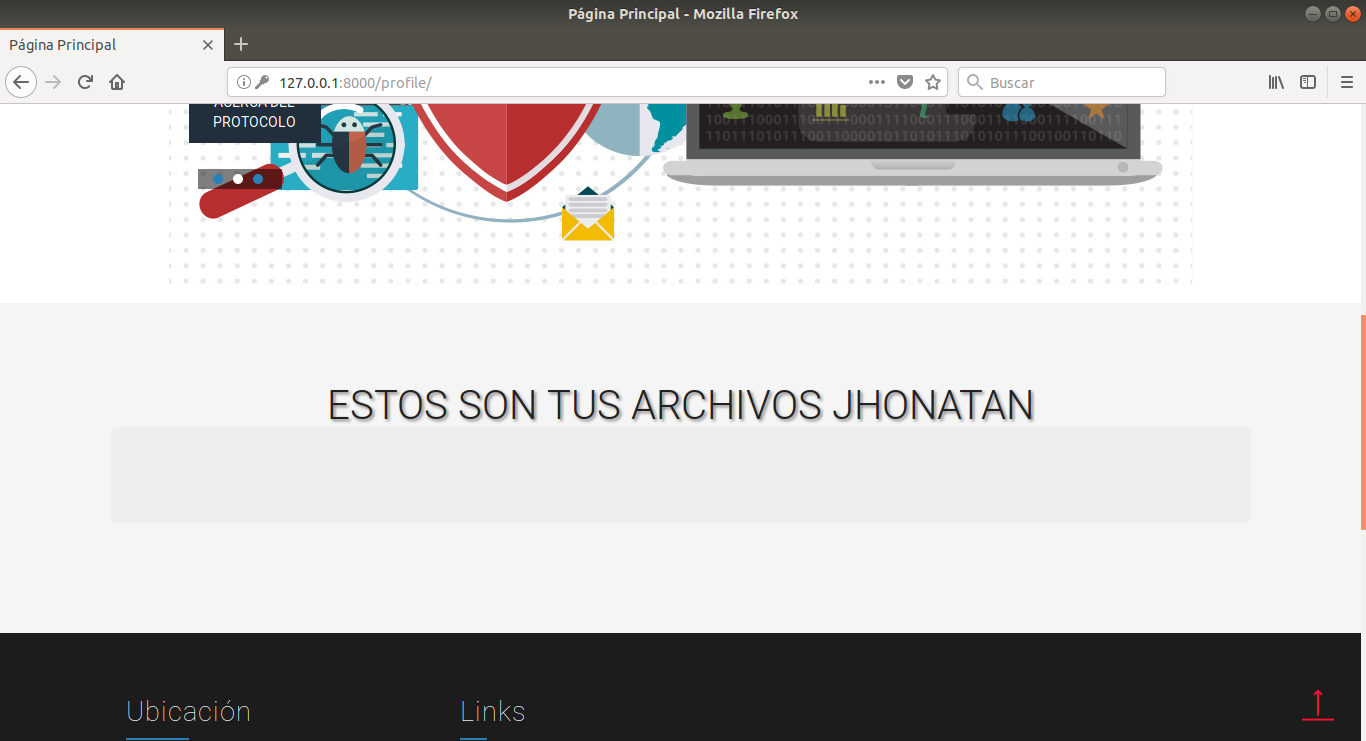
\includegraphics[width=14cm, height=7.5cm]{./images/Implementacion/PerfilOtroUsuario.png}
			\caption{Pantalla de Perfil.}
			\label{fig:6-1-20} 
			\end{figure}

\subsubsection{Subir Archivo}

			\begin{figure}[H]
			\centering
			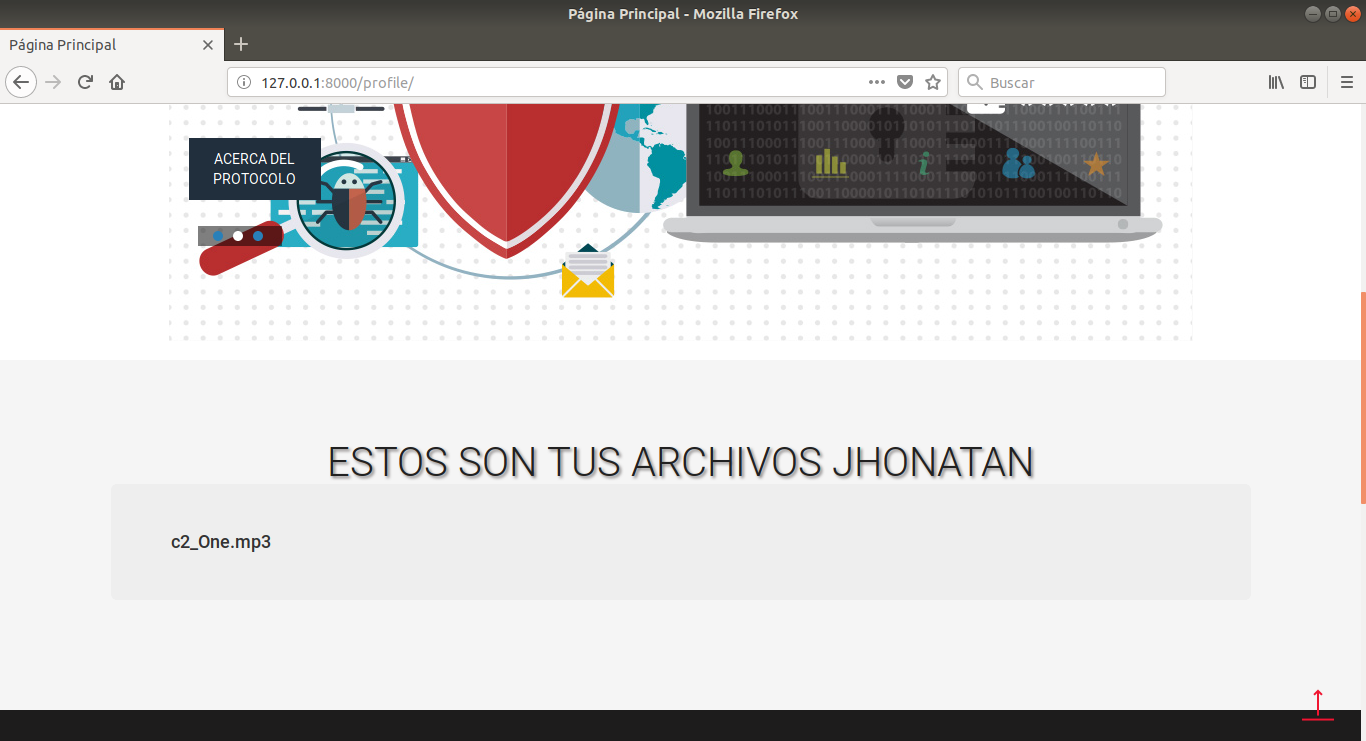
\includegraphics[width=14cm, height=7.5cm]{./images/Implementacion/SubirArchivoOtroUsuario.png}
			\caption{Pantalla de Perfil actualizada ya que el usuario subió un archivo, como es un duplicado sólo se guarda el c2 de dicho archivo.}
			\label{fig:6-1-21} 
			\end{figure}

\subsubsection{Tabla Cipher actualizada}

			\begin{figure}[H]
			\centering
			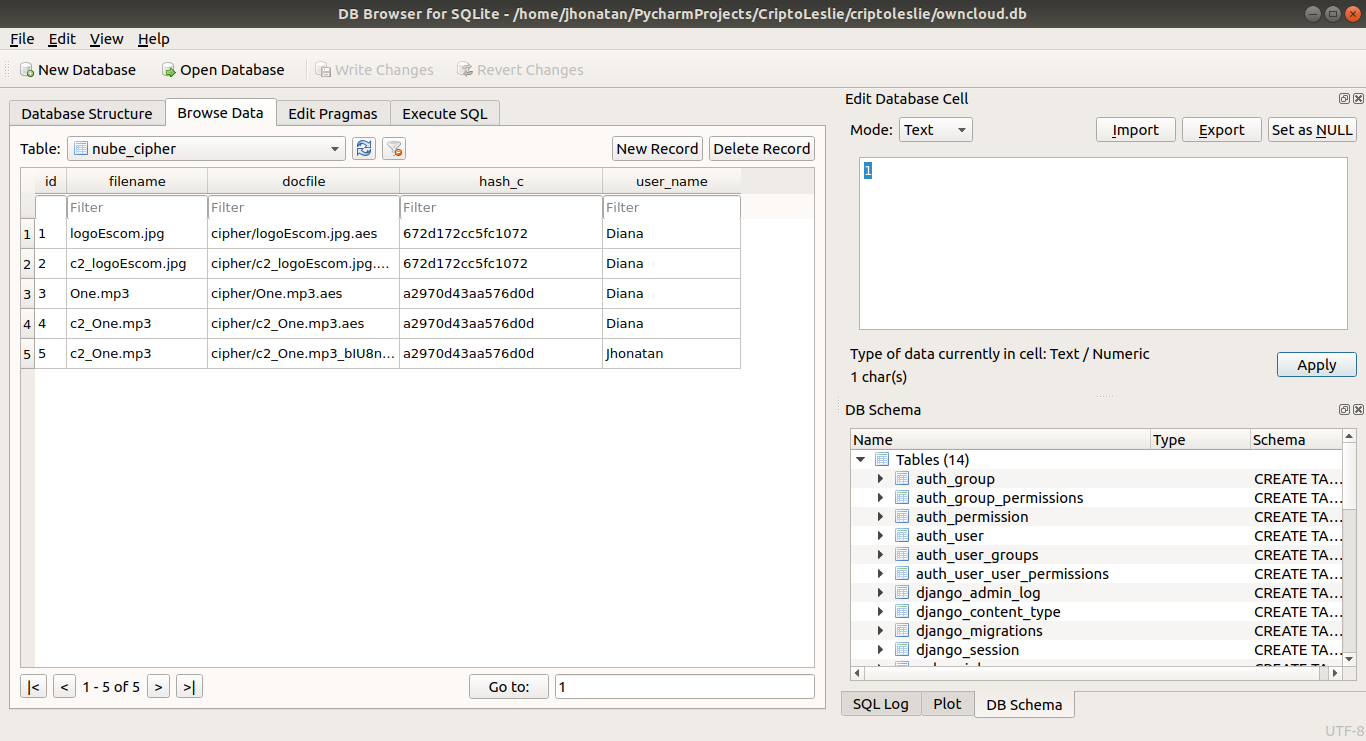
\includegraphics[width=14cm, height=7.5cm]{./images/Implementacion/TablaCipherOtroUsuario.png}
			\caption{Tabla Cipher actualizada.}
			\label{fig:6-1-22} 
			\end{figure}

\subsubsection{Tabla Hashes actualizada}

			\begin{figure}[H]
			\centering
			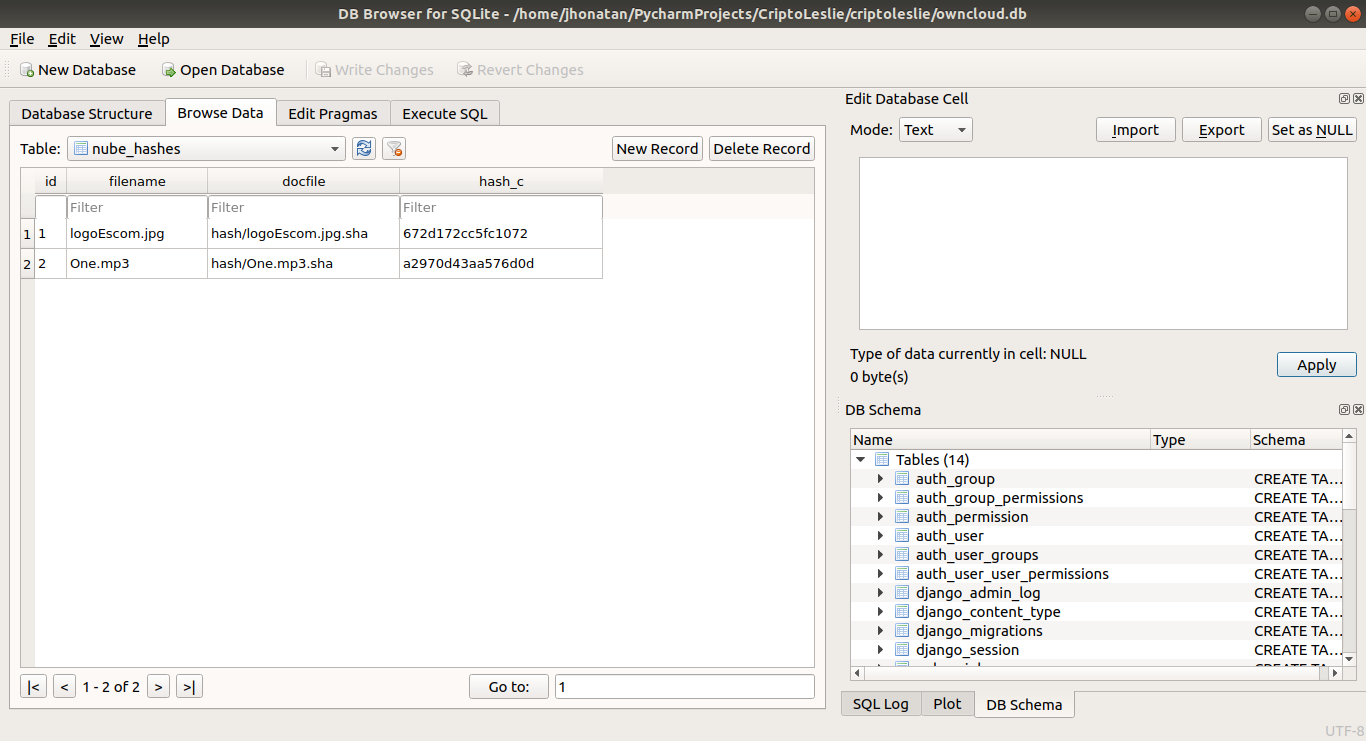
\includegraphics[width=14cm, height=7.5cm]{./images/Implementacion/TablaHashesOtroUsuario.png}
			\caption{Tabla Hashes actualizada.}
			\label{fig:6-1-23} 
			\end{figure}

\subsubsection{Perfil Actualizado}

			\begin{figure}[H]
			\centering
			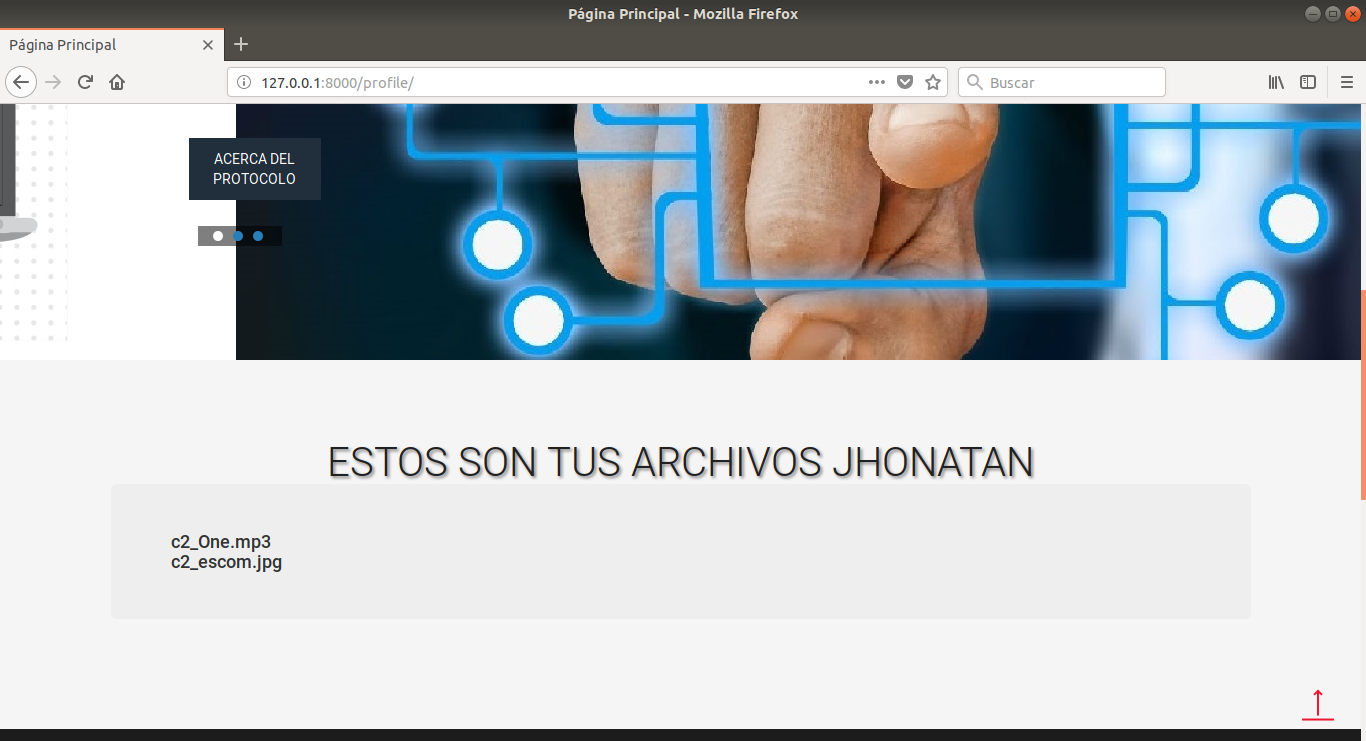
\includegraphics[width=14cm, height=7.5cm]{./images/Implementacion/PerfilOtroUsuarioActualizado.png}
			\caption{Perfil actualizado ya que el nuevo usuario subió más archivos.}
			\label{fig:6-1-24} 
			\end{figure}

\subsubsection{Tabla Cipher actualizada}

			\begin{figure}[H]
			\centering
			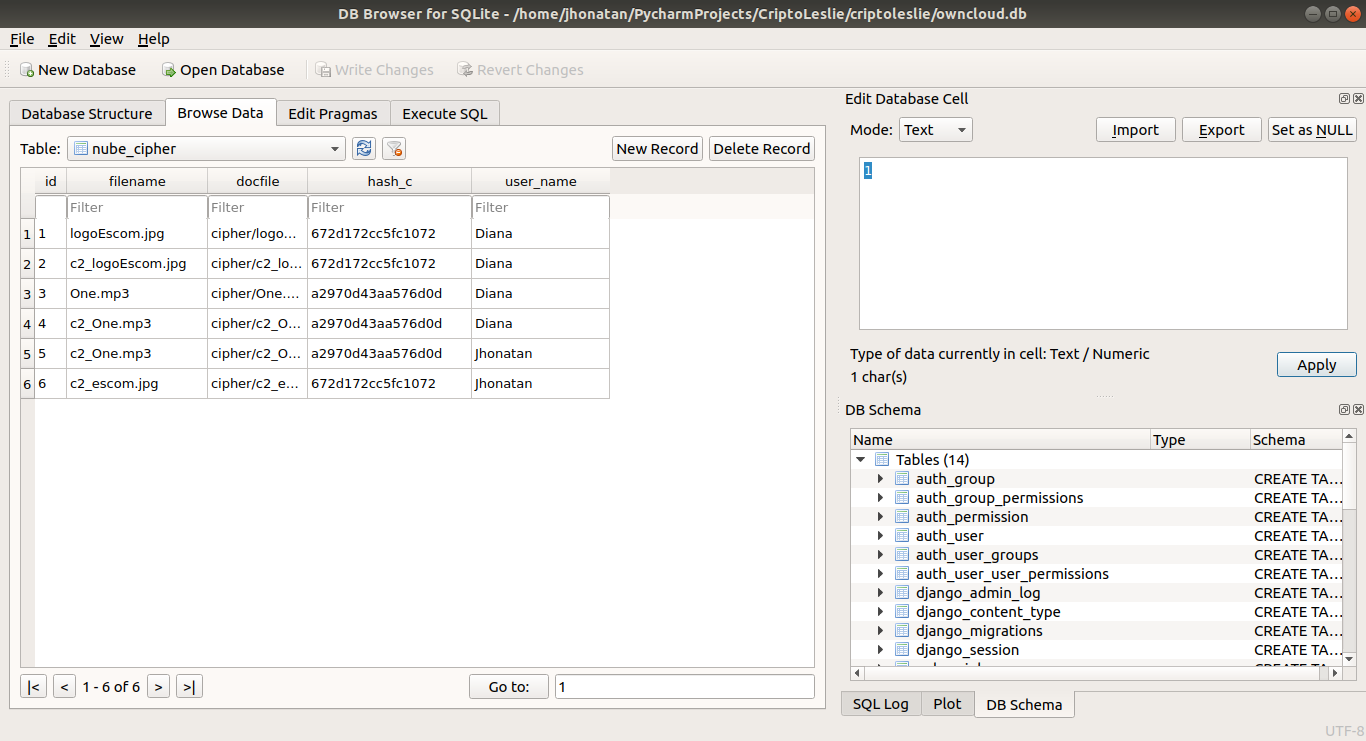
\includegraphics[width=14cm, height=7.5cm]{./images/Implementacion/TablaCipherOtroUsuarioActualizada.png}
			\caption{Tabla Cipher actualizada.}
			\label{fig:6-1-25} 
			\end{figure}

\subsubsection{Tabla Hashes actualizada}

			\begin{figure}[H]
			\centering
			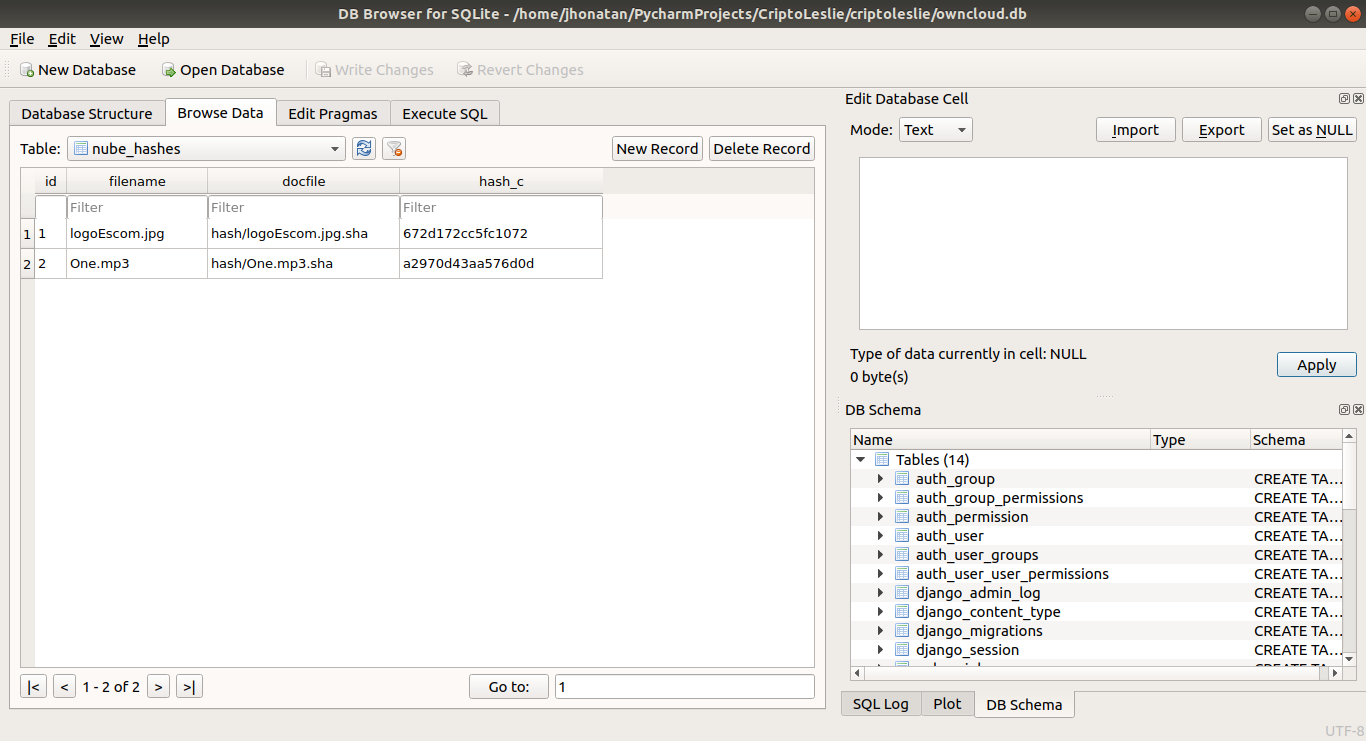
\includegraphics[width=14cm, height=7.5cm]{./images/Implementacion/TablaHashesOtroUsuarioActualizada.png}
			\caption{Tabla Hashes actualizada.}
			\label{fig:6-1-26} 
			\end{figure}

\subsection{Perfil de usuario1 actualizado con distintos formatos de archivos}

			\begin{figure}[H]
			\centering
			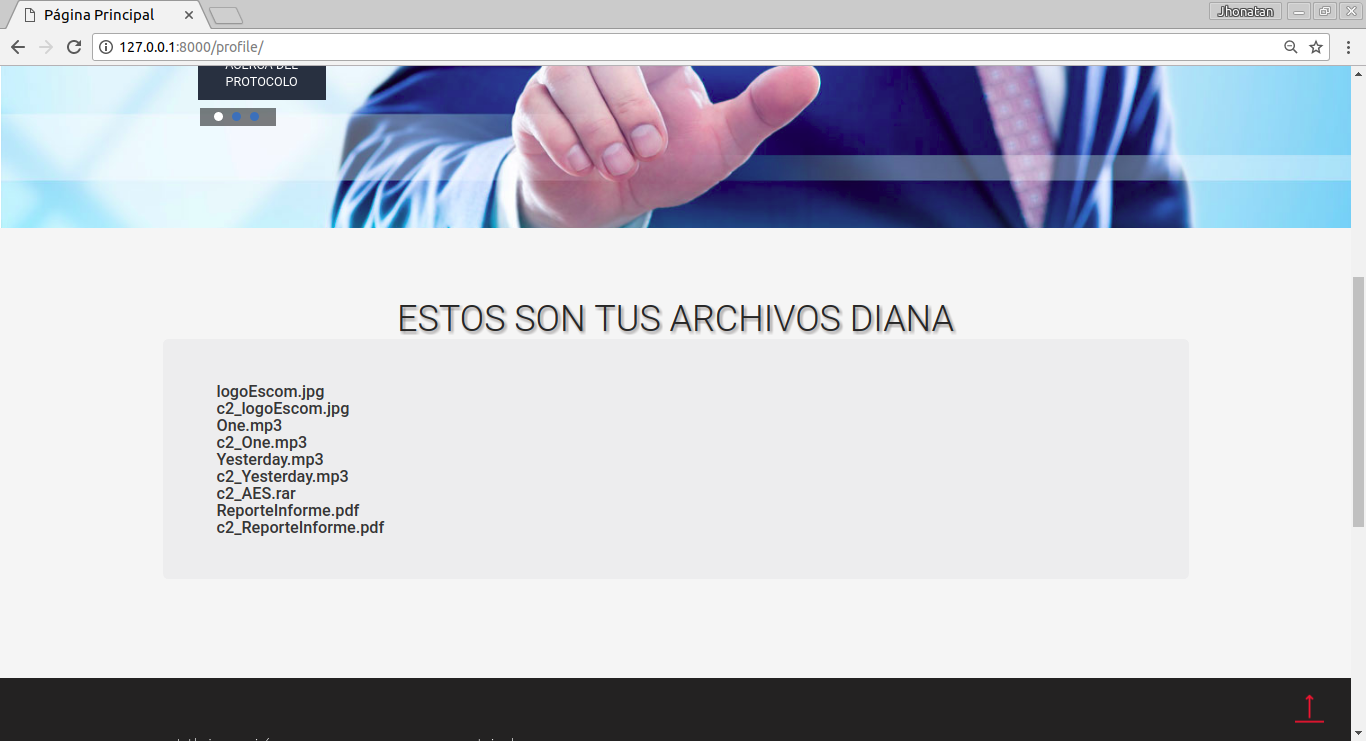
\includegraphics[width=14cm, height=7.5cm]{./images/Implementacion/PerfilUsuarioActualizado.png}
			\caption{Pantalla donde se muestran distintos tipos de archivos cifrados almacenados en la nube.}
			\label{fig:6-1-27} 
			\end{figure}

\subsubsection{Perfil de usuario2 actualizado con distintos formatos de archivos}

			\begin{figure}[H]
			\centering
			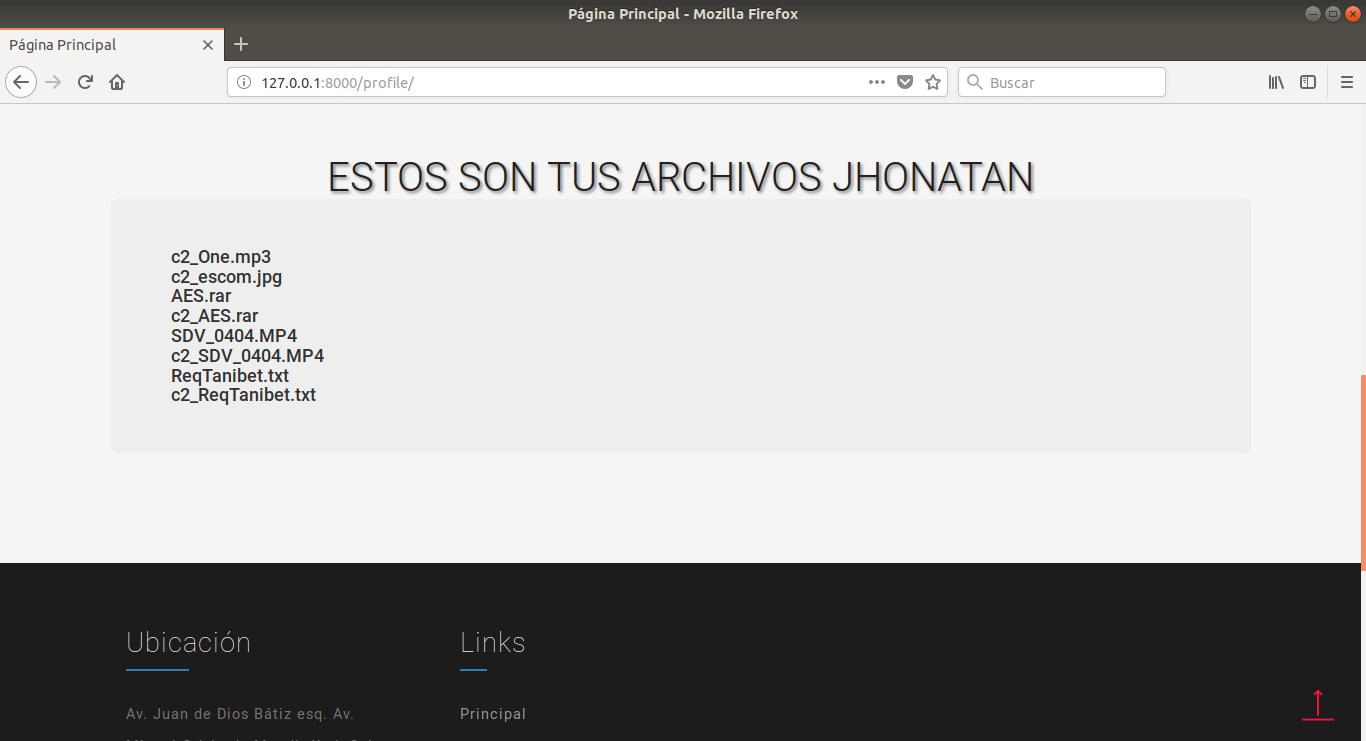
\includegraphics[width=14cm, height=7.5cm]{./images/Implementacion/PerfilJhonaActualizado.png}
			\caption{Pantalla donde se muestran distintos tipos de archivos cifrados almacenados en la nube.}
			\label{fig:6-1-28} 
			\end{figure}

\subsubsection{Tabla Cipher actualizada}

			\begin{figure}[H]
			\centering
			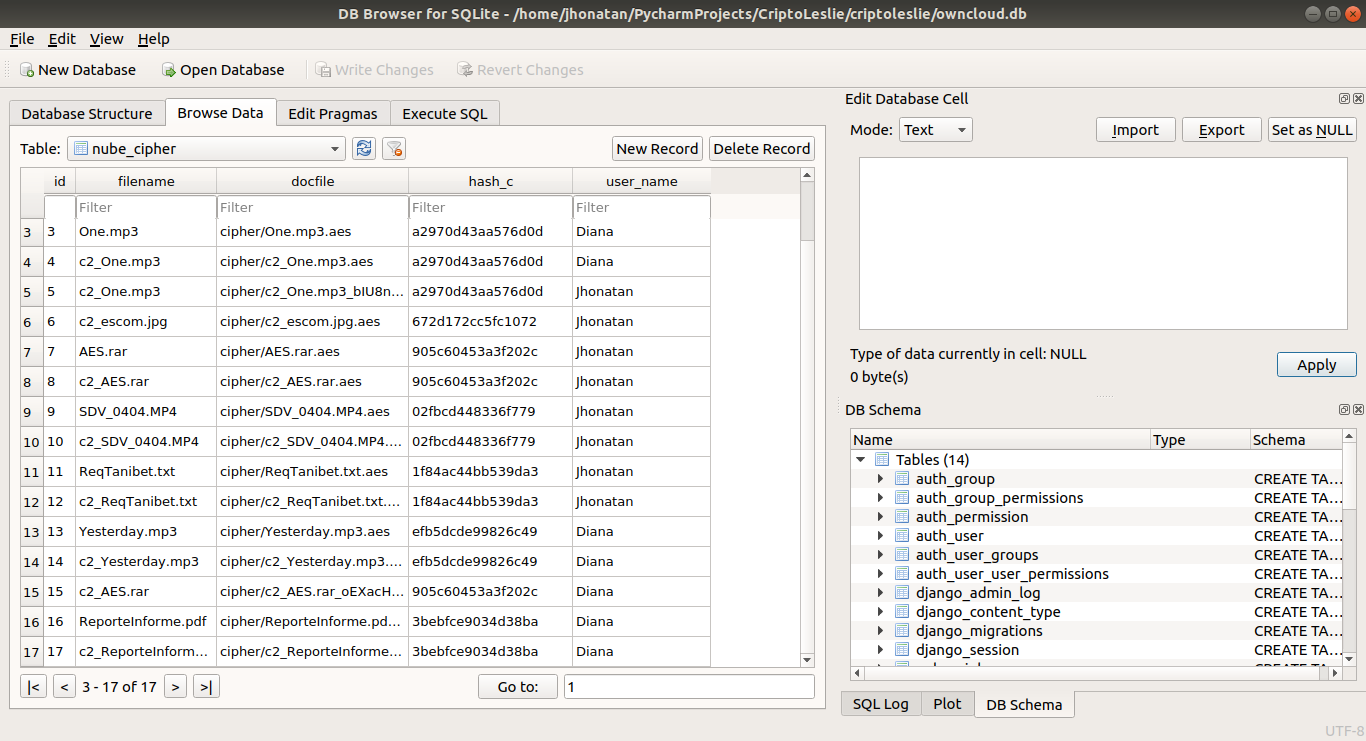
\includegraphics[width=14cm, height=7.5cm]{./images/Implementacion/CipherActualizada.png}
			\caption{Tabla Cipher actualizada.}
			\label{fig:6-1-29} 
			\end{figure}

\subsubsection{Tabla Hashes actualizada}

			\begin{figure}[H]
			\centering
			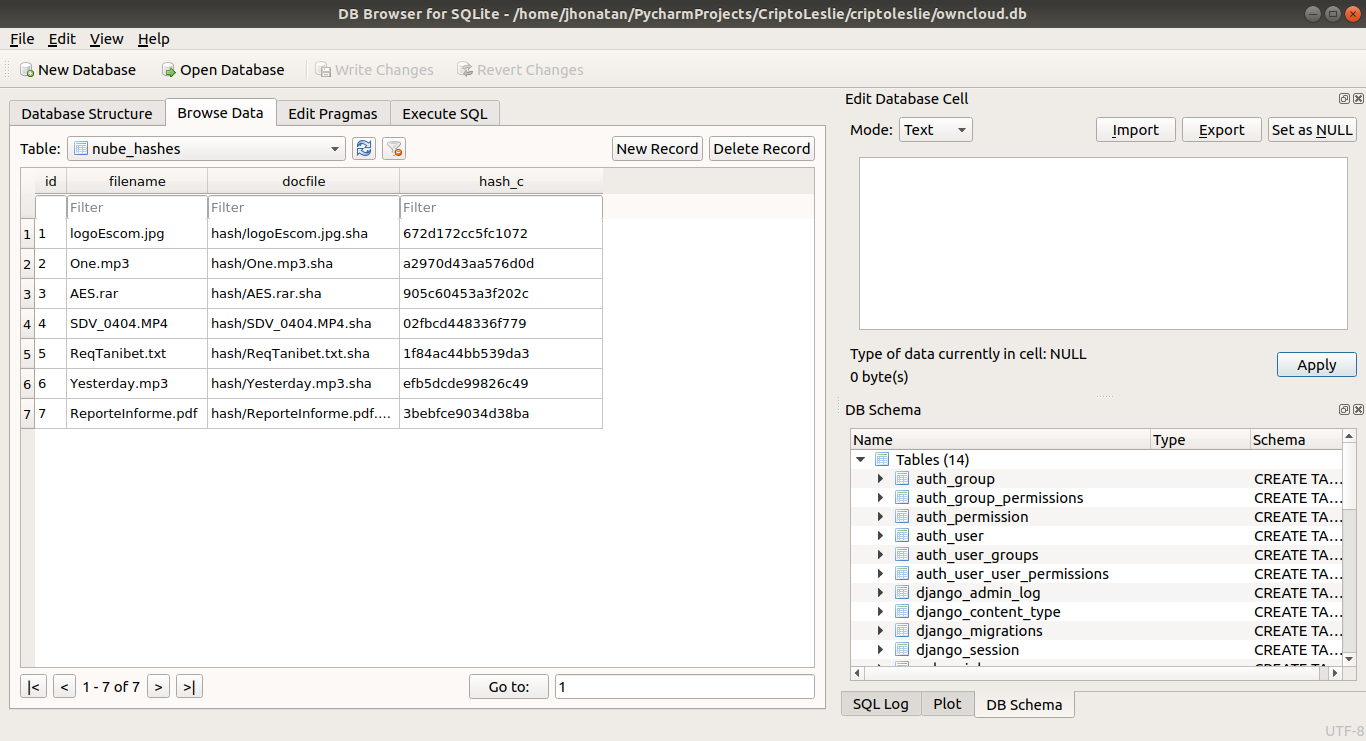
\includegraphics[width=14cm, height=7.5cm]{./images/Implementacion/HashesActualizada.png}
			\caption{Tabla Hashes actualizada.}
			\label{fig:6-1-30} 
			\end{figure}

\subsection{Descargar Archivo}

			\begin{figure}[H]
			\centering
			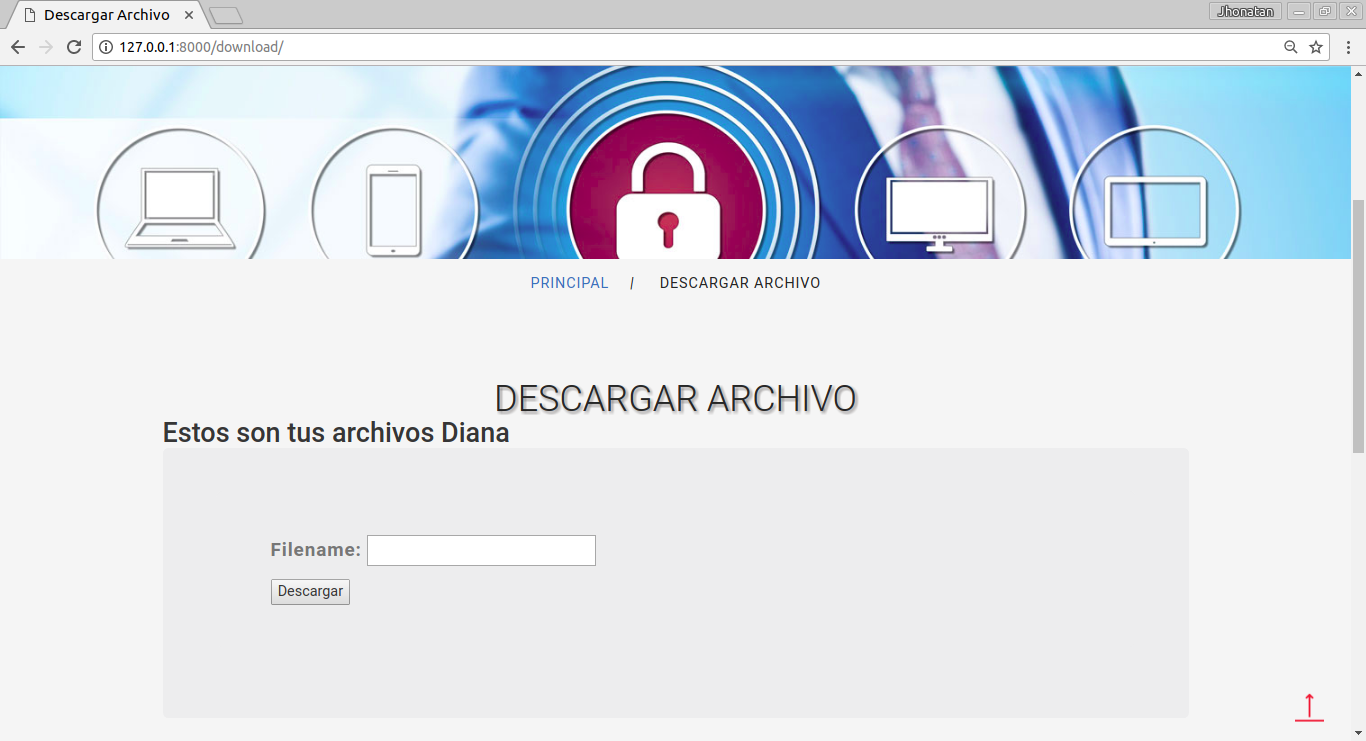
\includegraphics[width=14cm, height=7.5cm]{./images/Implementacion/DescargarArchivo.png}
			\caption{Pantalla donde se muestran el formulario donde se puede descargar los archivos.}
			\label{fig:6-1-31} 
			\end{figure}

\subsubsection{Seleccionando Archivo}

			\begin{figure}[H]
			\centering
			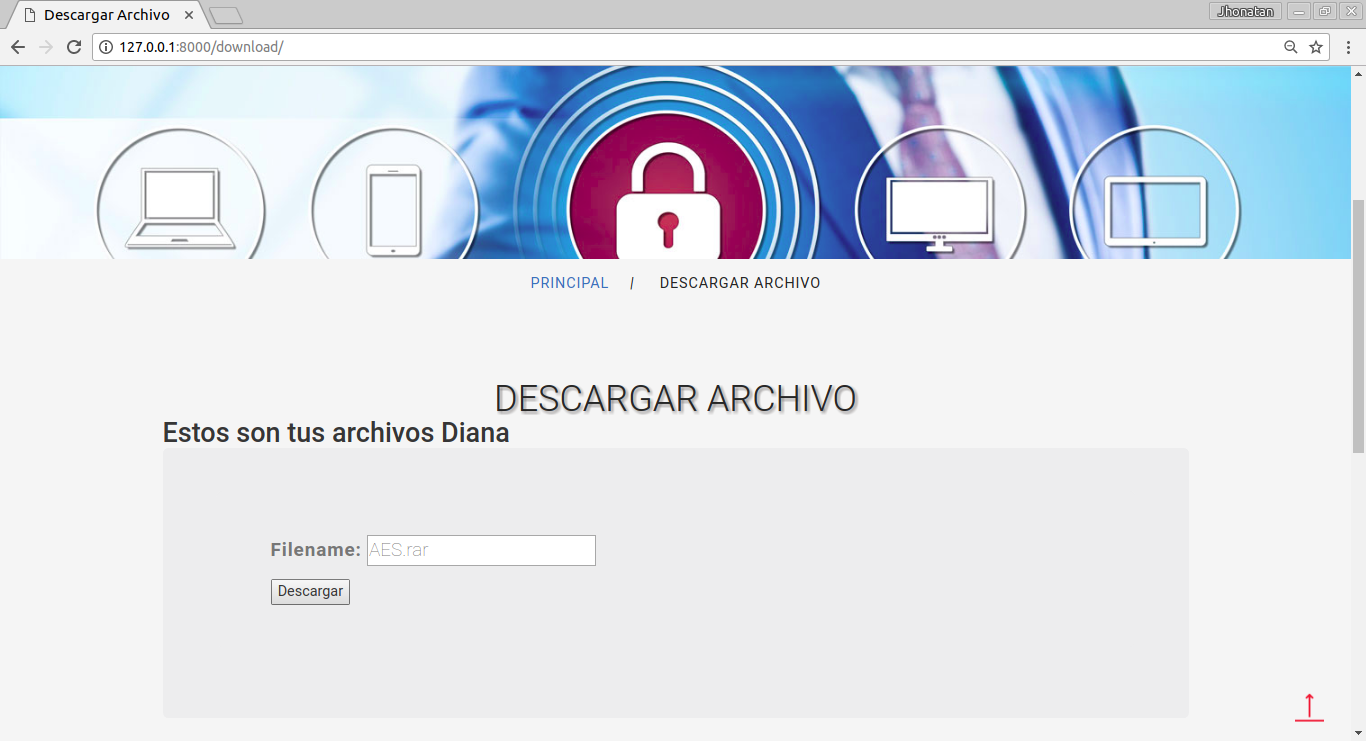
\includegraphics[width=14cm, height=7.5cm]{./images/Implementacion/DescargarArchivoSeleccionado.png}
			\caption{Pantalla donde se muestra el archivo seleccionado que se desea descargar.}
			\label{fig:6-1-32} 
			\end{figure}

\subsubsection{Archivo Descargado}

			\begin{figure}[H]
			\centering
			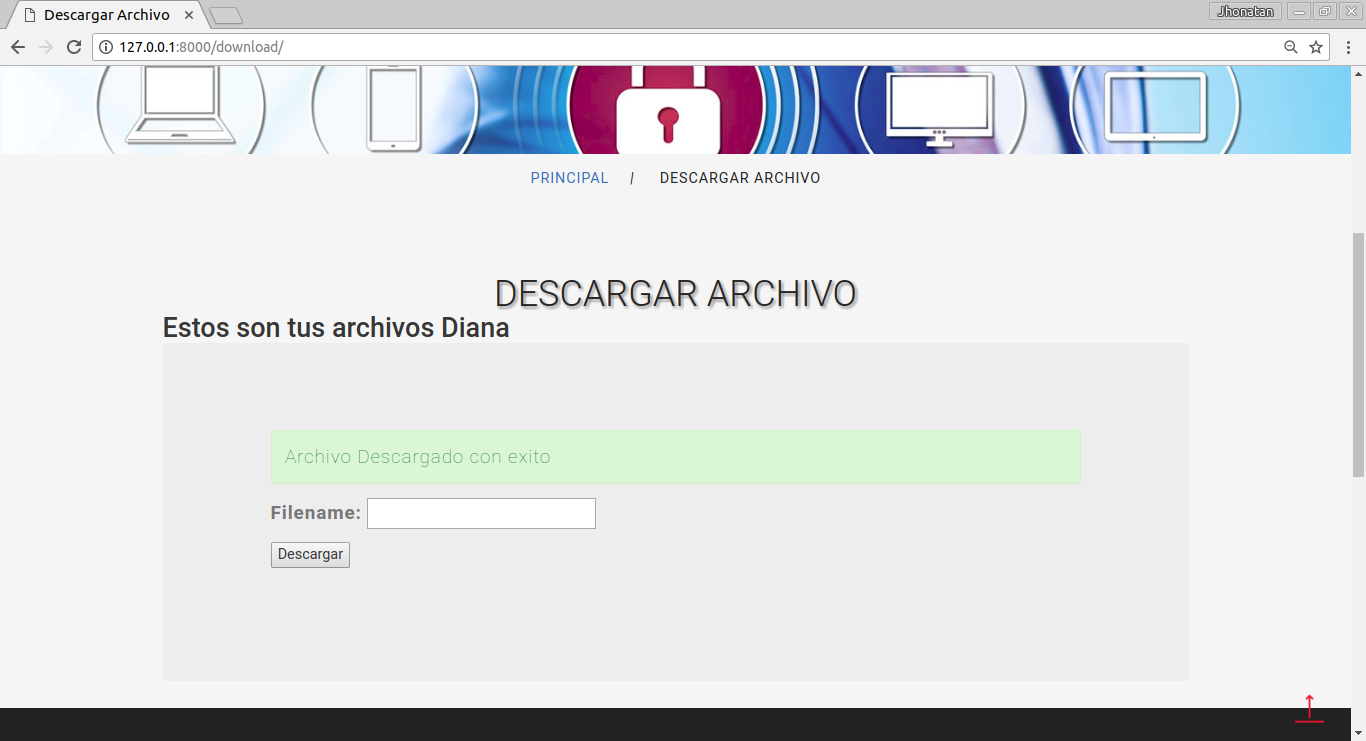
\includegraphics[width=14cm, height=7.5cm]{./images/Implementacion/DescargarArchivoOk.png}
			\caption{Pantalla donde se muestra que se descargo correctamente el archivo.}
			\label{fig:6-1-33} 
			\end{figure}

\subsubsection{Archivo Descargado en la Carpeta}

			\begin{figure}[H]
			\centering
			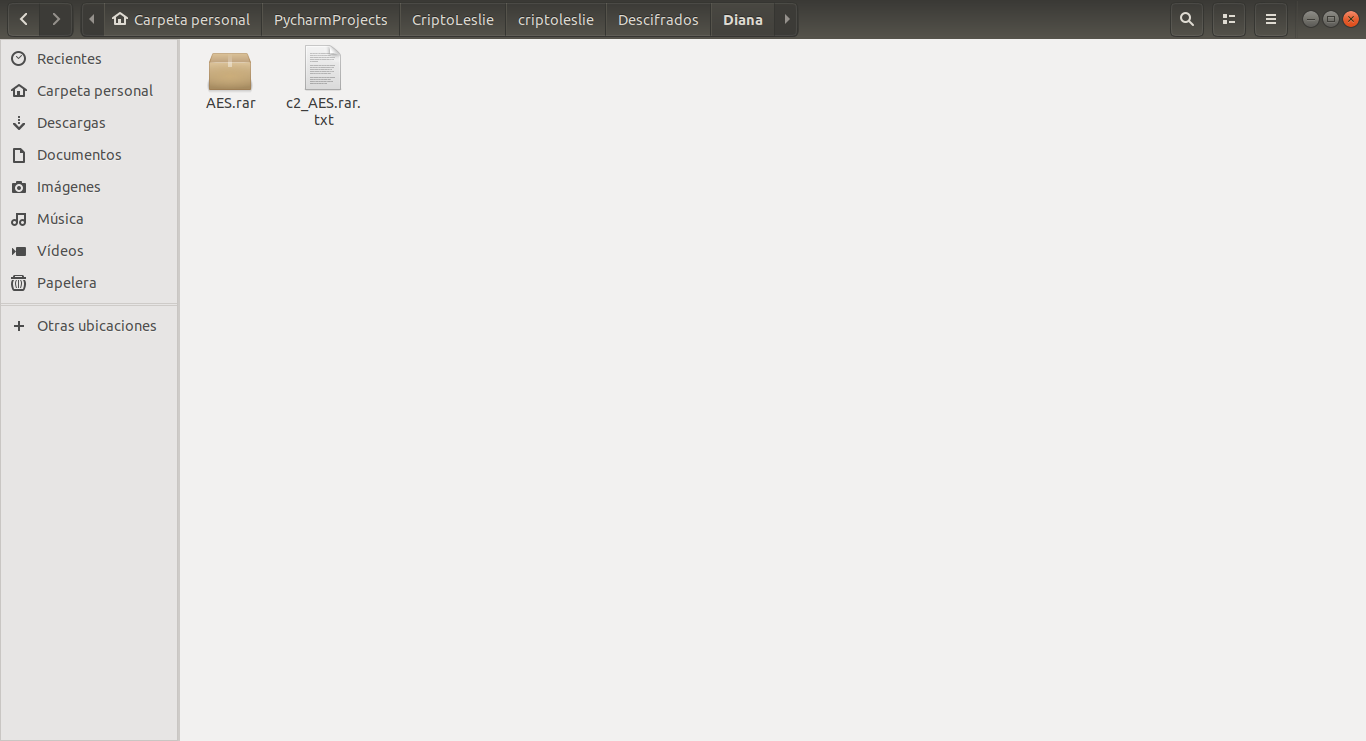
\includegraphics[width=14cm, height=7.5cm]{./images/Implementacion/DescargarArchivoCarpeta.png}
			\caption{Pantalla donde se muestra el archivo en la carpeta donde se descargo.}
			\label{fig:6-1-34} 
			\end{figure}

\subsubsection{Archivos Descargados del usuario 1 en la Carpeta}

			\begin{figure}[H]
			\centering
			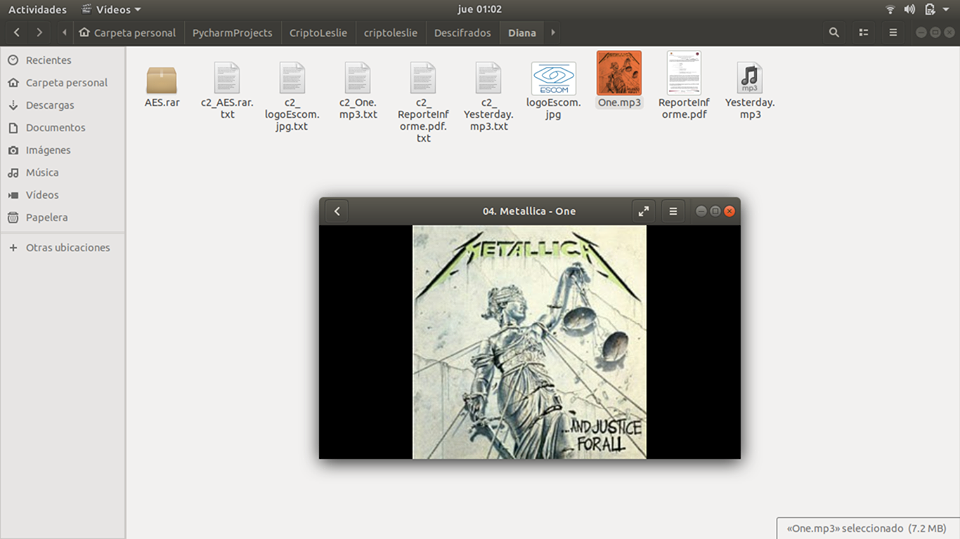
\includegraphics[width=14cm, height=7.5cm]{./images/Implementacion/DescargarArchivoCarpeta2.png}
			\caption{Pantalla donde se muestran los archivos en la carpeta donde se descargo del usuario 1.}
			\label{fig:6-1-34} 
			\end{figure}

\subsubsection{Archivos Descargados del usuario 2 en la Carpeta}

			\begin{figure}[H]
			\centering
			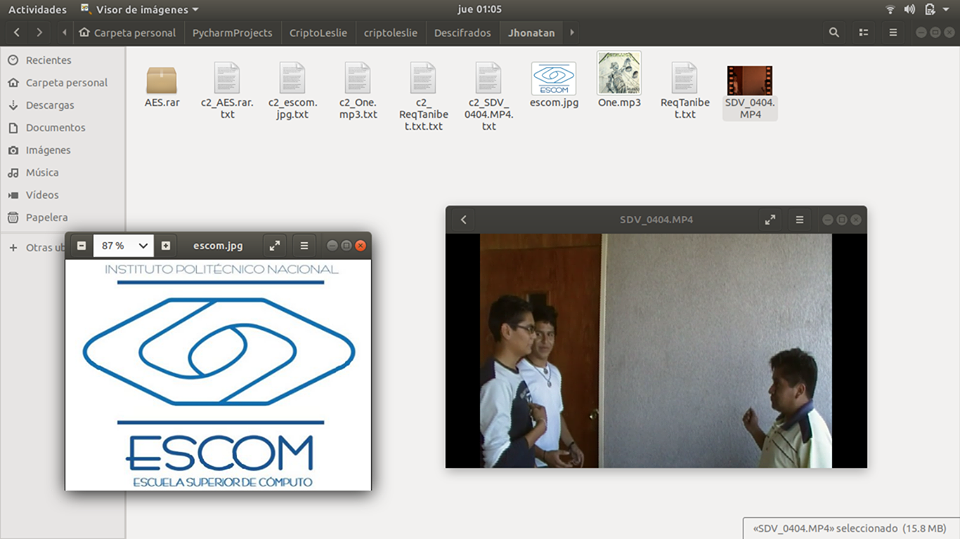
\includegraphics[width=14cm, height=7.5cm]{./images/Implementacion/DescargarArchivoCarpeta3.png}
			\caption{Pantalla donde se muestran los archivos en la carpeta donde se descargo del usuario 2.}
			\label{fig:6-1-35} 
			\end{figure}

\subsection{Eliminar Archivo}

			\begin{figure}[H]
			\centering
			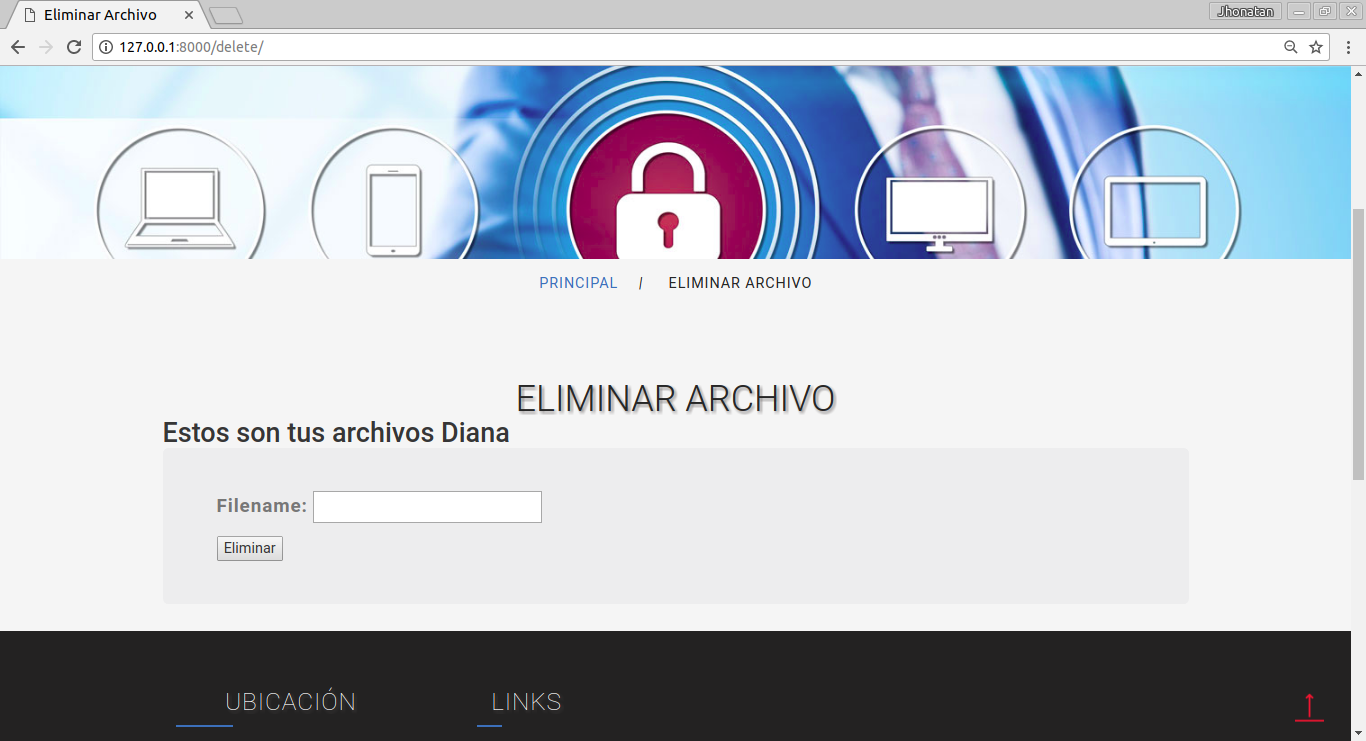
\includegraphics[width=14cm, height=7.5cm]{./images/Implementacion/EliminarArchivo.png}
			\caption{Pantalla donde se muestra el formulario donde se puede elimnar un archivo.}
			\label{fig:6-1-36} 
			\end{figure}

\subsubsection{Seleccionando Archivo a eliminar}

			\begin{figure}[H]
			\centering
			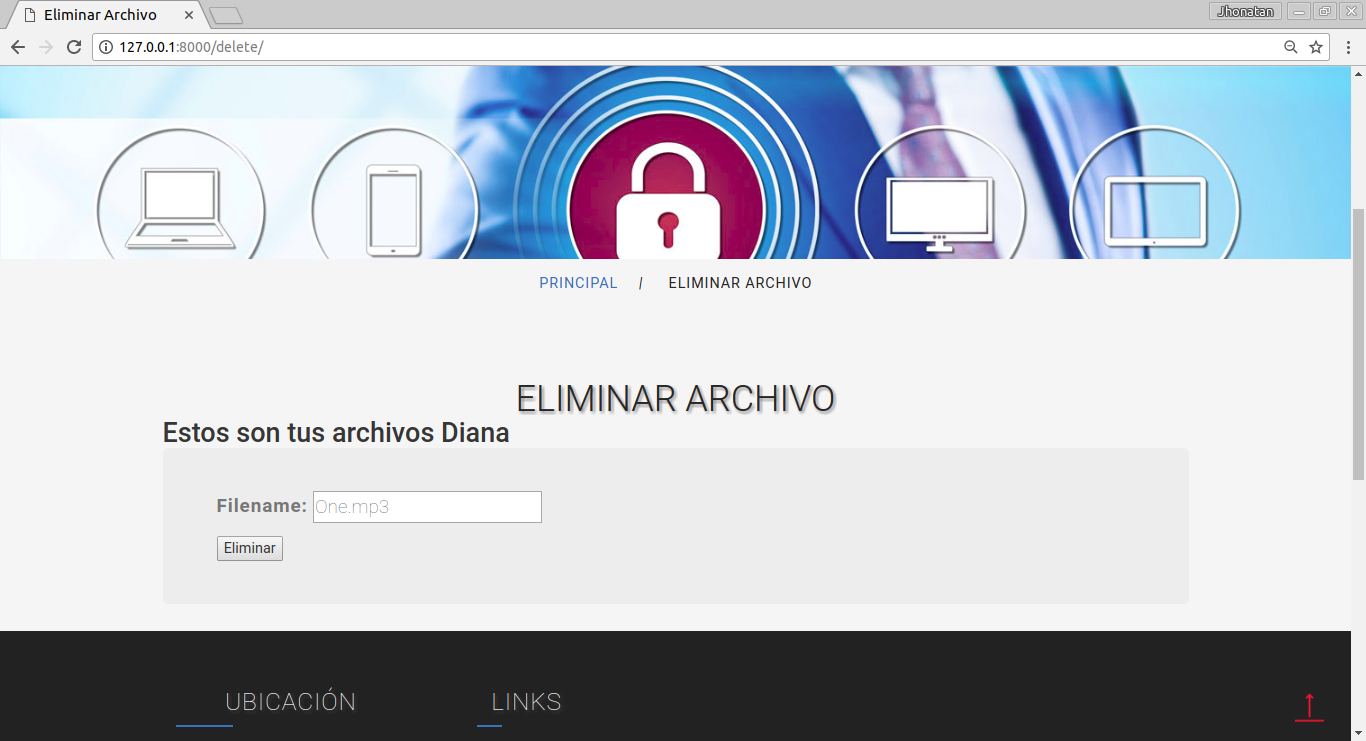
\includegraphics[width=14cm, height=7.5cm]{./images/Implementacion/EliminarArchivoSeleccionado.png}
			\caption{Pantalla donde se muestra el formulario donde se eligió un archivo a eliminar.}
			\label{fig:6-1-37} 
			\end{figure}

\subsubsection{Tabla Cipher con Archivo eliminado de usuario 1}

			\begin{figure}[H]
			\centering
			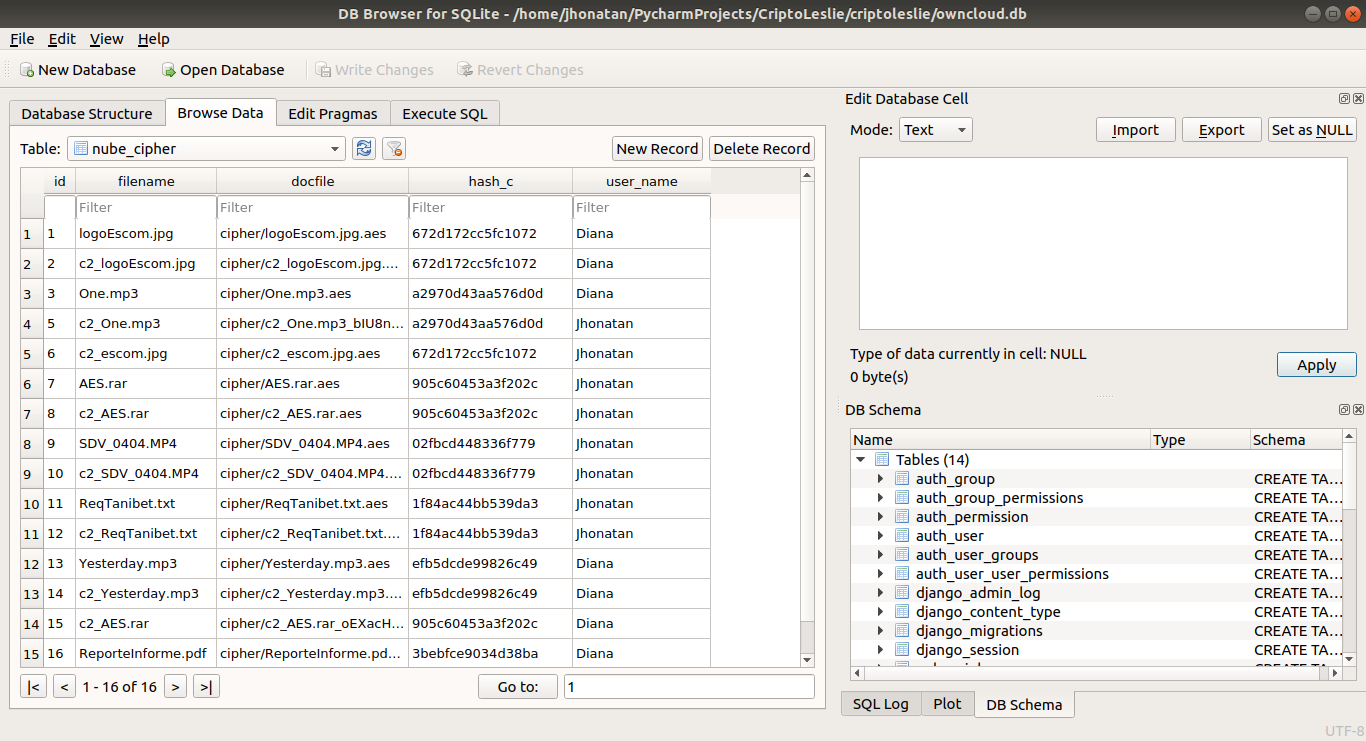
\includegraphics[width=14cm, height=7.5cm]{./images/Implementacion/TablaCipherArchivoEliminado.png}
			\caption{Pantalla donde se muestra la base de datos ya con el archivo eliminado.}
			\label{fig:6-1-38} 
			\end{figure}

\subsubsection{Pantalla archivos actualizados}

			\begin{figure}[H]
			\centering
			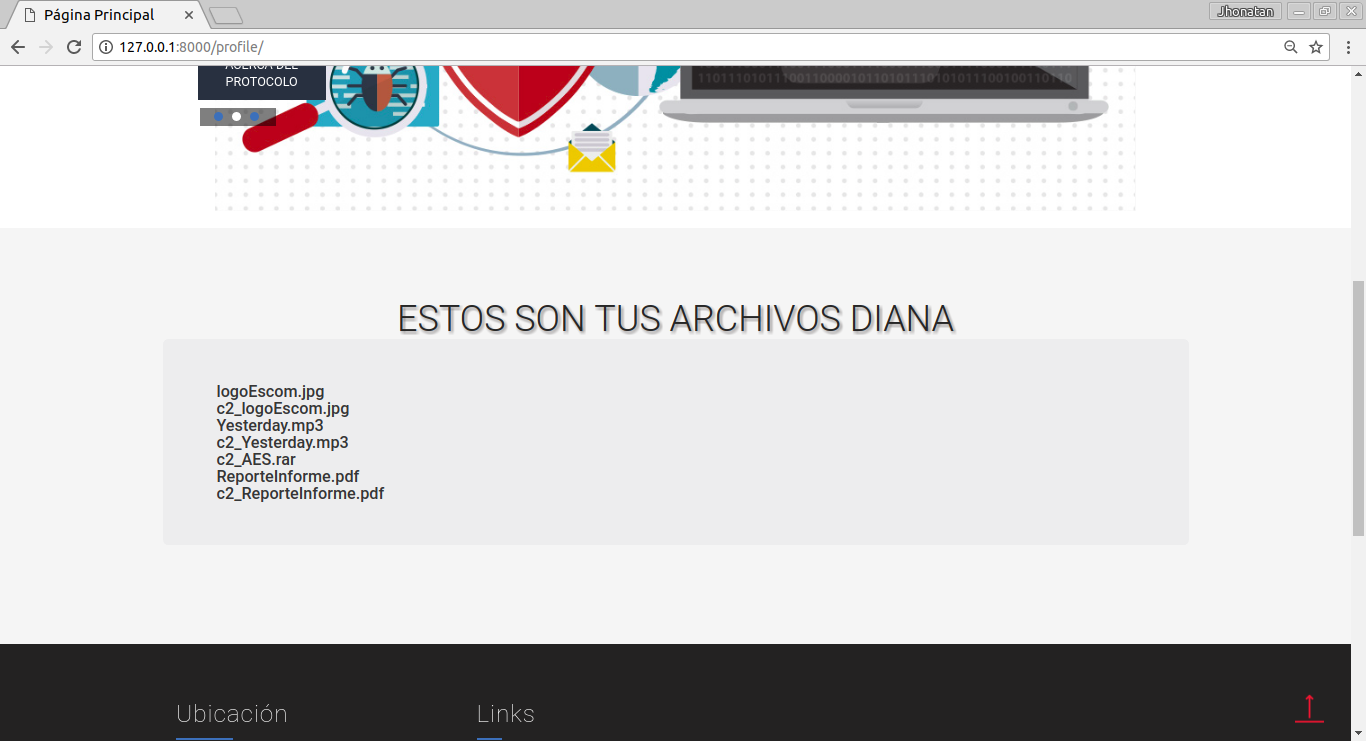
\includegraphics[width=14cm, height=7.5cm]{./images/Implementacion/ArchivoEliminado.png}
			\caption{Pantalla donde se muestra la lista de archivos actualizada despues de eliminar el archivo.}
			\label{fig:6-1-39} 
			\end{figure}

\subsubsection{Tabla Cipher con Archivo eliminado de usuario 2}

			\begin{figure}[H]
			\centering
			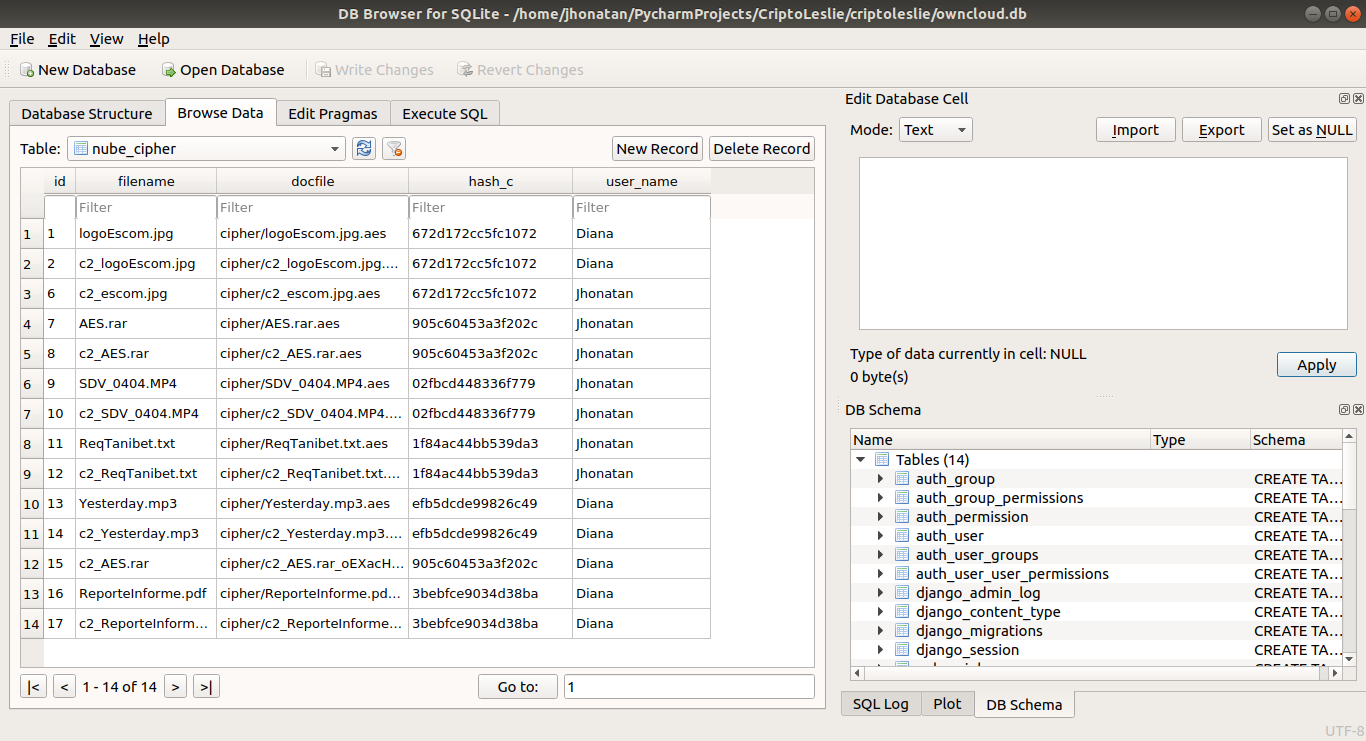
\includegraphics[width=14cm, height=7.5cm]{./images/Implementacion/TablaCipherArchivoEliminado2.png}
			\caption{Pantalla donde se muestra la base de datos ya con el archivo eliminado en los dos usuarios.}
			\label{fig:6-1-40} 
			\end{figure}

\subsubsection{Pantalla archivos actualizados de usuario 2}

			\begin{figure}[H]
			\centering
			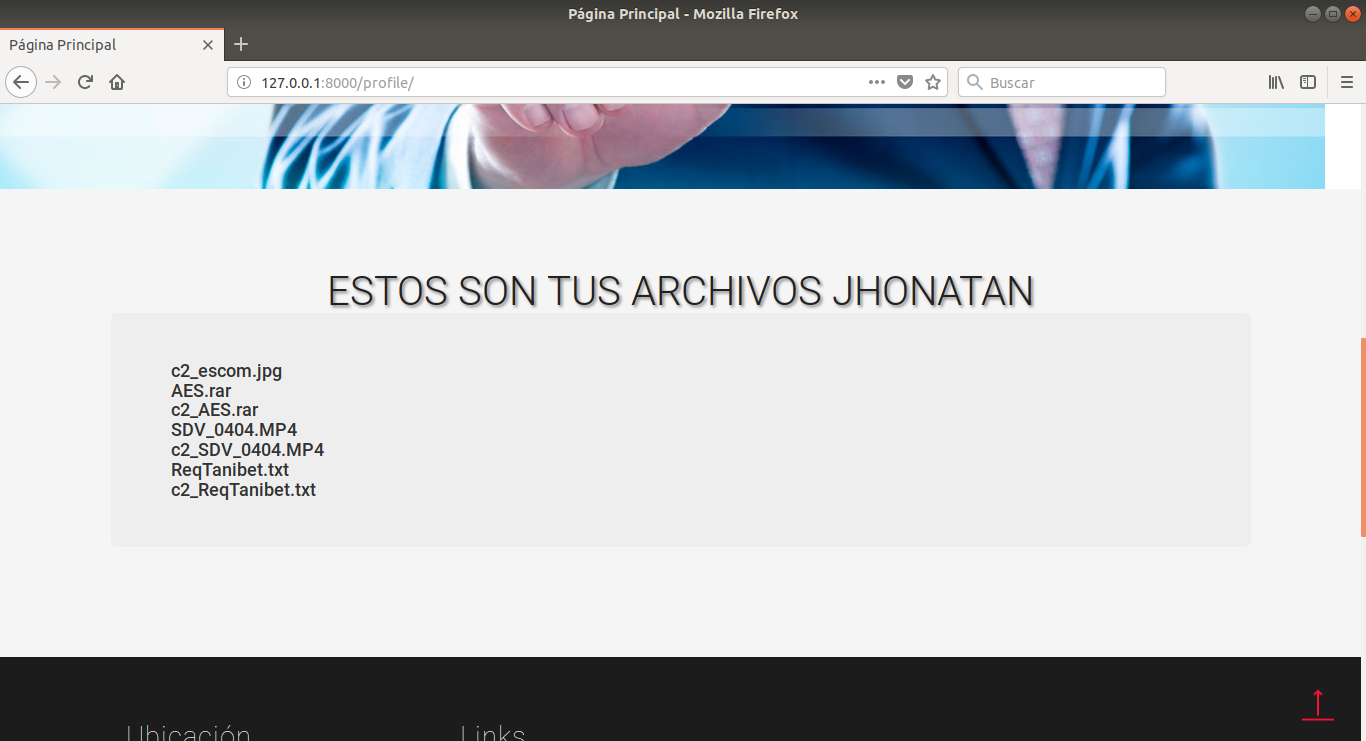
\includegraphics[width=14cm, height=7.5cm]{./images/Implementacion/ArchivoEliminado2.png}
			\caption{Pantalla donde se muestra la lista de archivos actualizada despues de eliminar el archivo del usuario 2.}
			\label{fig:6-1-41} 
			\end{figure}

\subsubsection{Tabla Hashes con Archivo eliminado de los dos usuarios}

			\begin{figure}[H]
			\centering
			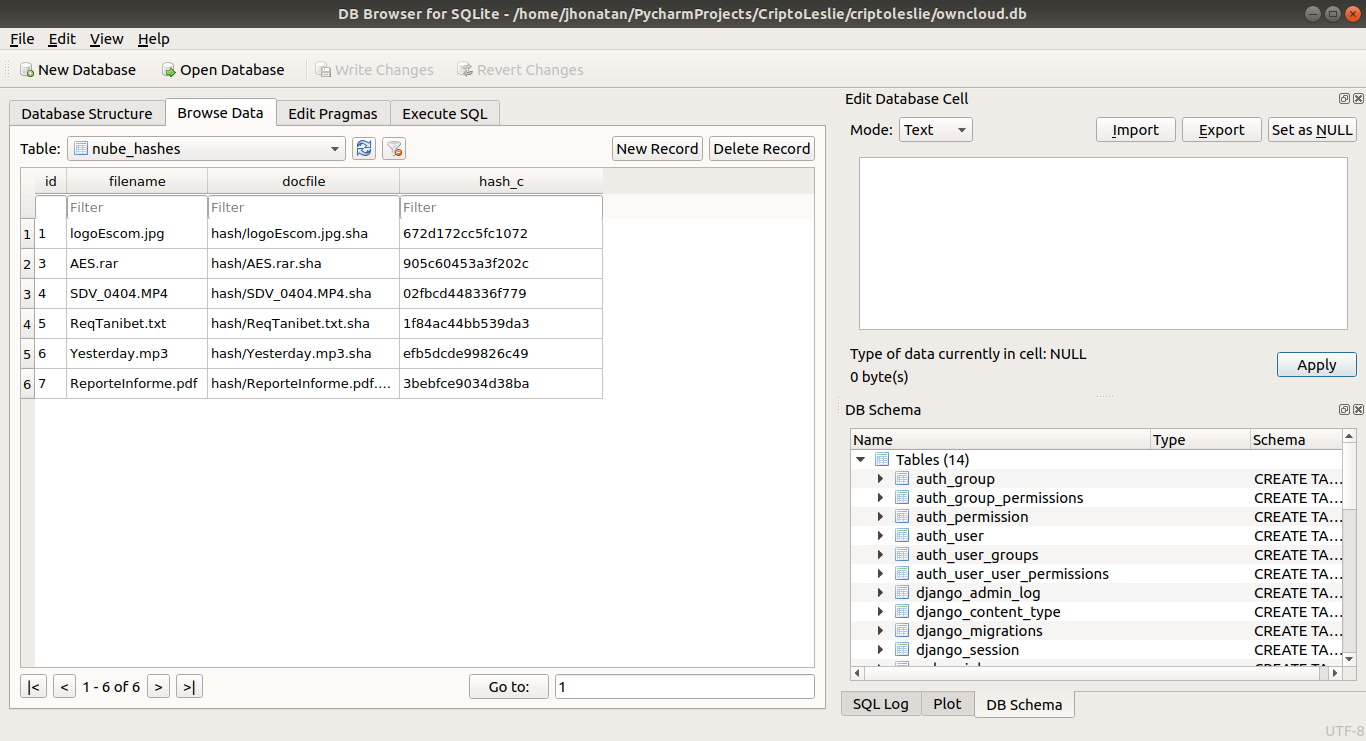
\includegraphics[width=14cm, height=7.5cm]{./images/Implementacion/TablaHashesArchivoEliminado.png}
			\caption{Pantalla donde se muestra la base de datos en la tabla de Hashes despues de haber eliminado un archivo por completo}
			\label{fig:6-1-42} 
			\end{figure}




